\documentclass{article}
\usepackage{graphicx}
\usepackage{hyperref}
\usepackage{amssymb}
\usepackage{amsmath}
\usepackage{amsthm}
\usepackage{algorithm}
\usepackage{algorithmic}
\usepackage{graphicx}  
\usepackage{caption}  
\usepackage{subcaption}
\usepackage{float}
\usepackage[a4paper, total={6in, 8in}]{geometry}

\usepackage[style = authoryear, backend = biber]{biblatex}
\addbibresource{references.bib}

\DeclareFieldFormat{labelnumberwidth}{[#1]\adddot} % Adds numbered labels
\renewbibmacro{begentry}{\printfield{labelnumber}} % Ensures that the bibliography has numbers

%defining custom environments
\theoremstyle{definition}
\newtheorem{definition}{Definition}[section]
\newtheorem{claim}{Claim}
\newtheorem{lemma}{Lemma}
\newtheorem{proposition}{Proposition}
\newtheorem{theorem}{Theorem}

\begin{document}

% Cover Page
\begin{titlepage}
    \centering
    \vspace*{2cm}

    % Title
    {\Huge \textbf{Deep Hedging in Low-Data Environments using Path Signatures}} \\[1.5cm]

    % Author
    {\Large Author: Nick Bossi} \\[0.5cm]

    % Supervisors
    {\large Supervisor: Associate Professor Jonathan Shock} \\[0.5cm]
    {\large Co-Supervisor: Yuri Robbertze} \\[1.5cm]

    % Institution
    {\Large UCT Department of Mathematics and Applied Mathematics} \\[1.5cm]

    % Logo
    \includegraphics[width=0.4\textwidth]{UCT_logo.png} \\[1.5cm] % Make sure to replace 'UCT_logo.png' with the correct filename

    % Date
    {\large 27 September 2024}

    \vfill
\end{titlepage}
\newpage

\tableofcontents
\newpage
\listoffigures
\listoftables

\newpage
\section{Abstract}
Historically, many approaches of hedging a financial derivative have been explored. This paper attempts to answer whether Deep Neural Networks (DNNs) can provide robust tools for the hedging of a European Best-of option. As we are using deep learning techniques, we face the issue of not having sufficient real-world data in order to effectively train our model. We thus employ the use of a Conditional Variational Autoencoder as a tool to learn the underlying stock's distributions so that we can simulate a range of psuedo-real-world future paths. The advantage of this is two-fold, as it provides realistic training data for our deep hedger, as well as giving us a theoretical means to test the robustness of our hedger under many future market conditions. Instead of directly using time-series stock data, we make use of a feature mapping for time-series data known as a path signature, which has been shown to effectively capture key information of the joint-distributions of temporal data. Our findings imply that the use of deep recurrent networks give promising results in that they on average give a more risk-neutral hedging strategy than strategies informed by the Black-Scholes model, although issues in variability were also found.
\newpage
\section{Acknowledgements}
I would like to thank Associate Professor Jonathan Shock for agreeing to supervise me on this project, for asking thought-provoking questions, and for offering guidance on the process of scientific writing.\\\\
I would also like to thank Jake Stangroom, who helped with path signature and VAE related questions, even when there was no obligation on his part to do so.\\\\
Special thanks must be given to Mr Yuri Robbertze, who went beyond the role of supervisor in helping me understand the topics involved in the project, and who's infectious zeal for all things maths continues to inspire me. \\\\
I would also like to express gratitude to the scientific community as a whole, whose publicly available publications and articles make learning so accessible, and whose resultant tools (such as ChatGPT) aid considerably in the learning and writing of scientific content.\\\\ 
Finally, and as always, I thank my mom and dad for their continued emotional and financial support. Without them, I would never have been able to pursue my love for mathematics at a tertiary level, and for that I am eternally grateful. 
\newpage
\section{Introduction}
In 1973, Fischer Black, Myron Scholes and Robert Merton devised a new and revolutionary model to price financial options (\cite{black1973pricing}). They proved that under certain conditions, one can perfectly hedge an option by buying and selling the underlying asset. The model posits that the price of stocks follows a geometric brownian motion with constant drift and volatility. As with many models, key assumptions were made that fail in reality. Amongst others, these assumptions included that the market is frictionless (no transaction costs), and that assets can be traded continuously in time. In reality assets cannot be traded continuously, and thus our trading strategy needs to somehow compensate for this fact, something which strategies informed by the Black-Scholes equations do not do.
\\\\
This paper aims to assert whether Deep Neural Networks (DNNs) can better manage portfolios containing the assets underlying a European Best-of option so as to hedge said option. More explicitly, can a neural network govern a trading strategy which will more closely track the value of a contingent claim than a trading strategy as motivated by the Block-Scholes equations. Due to the manner in which neural networks can infer complex relationships without explicit models of the underlying process, we hypothesise that by removing explicit model assumptions and the assumption of continuous trading, a neural network may be able to better hedge a financial instrument in the discrete-time case given that it does not have the restrictive assumptions of the Black-Scholes model.
\\\\
We also hypothesise that Recurrent Neural Networks will be better able to tackle this task than more standard Feed-Forward Networks, as they have memory mechanisms which is useful for any sequential task, and thus relevant to our task as we are dealing with options based on the time-series data of stocks.
\\\\
We would like to employ deep learning techniques in order to hedge a financial instrument. A big hurdle to overcome is the fact that there is only one historical realisation of a particular financial instrument, and deep-learning techniques require large amounts of data to perform well. To overcome this we will use a generative model to learn the underlying distribution of the instrument of interest and then generate many novel sample paths by sampling from this learnt distribution, thus enabling us to use more conventional deep learning techniques for the problem of hedging.
\\\\
An added benefit of the generation process is that we can determine how well our model does on pseudo-real unseen data which can give us an indication on the robustness of our deep hedger under possible future market conditions.
\\\\
The specific option we will be investigating is an Exotic European Best-of Basket Option of the form:
\label{our option}
\begin{align}
    &H = 100H^*\\
    &H^* = \text{max}\left\{\frac{S^{1}_{T}}{S^{1}_{0}}, \frac{S^{2}_{T}}{S^{2}_{0}}\right\}.
\end{align}
where $S_t^1$ and $S_t^2$ represent the prices of two stocks at a given time $t$.
\newpage

\section{Literature Review}
\subsection{Path Signatures}
A path signature is an infinite dimensional tensor containing iterated path integrals over the domain of multidimensional paths (sequential data) (\cite{chevyrev2016primer}). It helps capture complicated interactions between paths, as well as fundamental characteristics of individual paths, such as when events took place relative to one another, whilst not being influenced by the parameterisation of the paths (\cite{lyons2023signature}).
It can be viewed as a feature map of a stream of data, and is essentially unique for a given path (\cite{lyons2023signature}, \cite{boedihardjo2013uniqueness}, \cite{boedihardjo2014signature}).
Being a uniquely determined feature map, a natural question is to ask whether signatures can be used in a machine learning context, where feature extraction allows for more effective and efficient inference.
Indeed they have been used in multiple machine learning problems with optimistic results. One successful application has been their use in classifying Chinese Characters, where the incorporation of terms from the path signature as features to a deep convolutional neural network (CNN) showed significant improvement in predictive capabilities (\cite{chinesecharacters}).
\subsubsection{Paths}
\begin{definition} 
A $d$-dimensional path $X:[a,b] \rightarrow \mathbb{R}^{d}$ is a continuous mapping from an interval of $\mathbb{R}, [a,b]$, to $\mathbb{R}^{d}$. Where $X_{t}$ denotes $X(t)$ for $t \in [a,b]$.\\\\
Alternatively we can view a $d$-dimensional path as a collection: 
$$X_{t} = (X_{t}^1,X_{t}^2,...,X_{t}^d),$$ where $X^i:[a,b] \rightarrow \mathbb{R}$ is a one-dimensional path for $\forall i \in \{1,...,d\}$.
\end{definition}
\begin{definition}
Given a one-dimension path $X:[a,b] \rightarrow \mathbb{R}$, the \textit{length} of $X$ is denoted
\begin{align}
    |X| := \sup_{P\subset [a,b]} \sum_{i=1}^{n} |X_{t_{i}}-X_{t_{i-1}}|
\end{align}
where the supremum is taken over all finite partitions $P = \{x_{1},...,x_{n}\}$ in $[a,b]$. \\\\
A $d$-dimensional path 
$X = (X^1,X^2,...,X^d),$ is said to be of \textit{bounded/finite variation} if $|X^i|$ is finite $\forall i \in \{1,...,d\}$.  
\end{definition}

\begin{definition}
    Given a path of bounded variation $X:[a,b] \rightarrow \mathbb{R}$ and a function $f: \mathbb{R} \rightarrow \mathbb{R}$, the integral of $f$ with respect to $X$ over $[a,b]$ is defined by:
    \begin{align}
      \int_{a}^{b} f(X_{t}) d X_{t} = \int_{a}^{b} f(X_{t}) \frac{d X_{t}}{d t} d t.  
    \end{align}
\end{definition}


\subsubsection{Path Signatures}
\begin{definition}
Given a $d$-dimensional path of bounded variation, $X:[a,b] \rightarrow \mathbb{R}^{d}$, and recalling that for $\forall i \in \{1,...,d\}$, $ X^i:[a,b] \rightarrow \mathbb{R}$ is a one-dimensional path. For all $i \in \{1,...,d\}$ we define the integral
\begin{align}
    S(X)_{a,t}^{i} = \int_{a<s<t} d X_{s}^{i} = X_{t}^{i} - X_{a}^{i}.
\end{align}
Similarly, for any pair $i,j \in \{1,...,d\}$ we define the double integral
\begin{align}
    S(X)_{a,t}^{i,j} = \int_{a<s<t} S(X)_{a,s}^{i} d X_{s}^{j} = \int_{a<s<t} \int_{a<r<s} d X_{r}^{i} 
 d X_{s}^{j} = \int_{a<r<s<t} d X_{r}^{i} d X_{s}^{j}.
\end{align}
 Continuing recursively, for any $k\geq 1$, and $i_{1}, i_{2}, ..., i_{k} \in \{1,...,d\}$, we define the iterated integral
 \begin{align}
   S(X)_{a,t}^{i_{1},...,i_{k}} = \int_{a<s<t} S(X)_{a,t}^{i_{1},...,i_{k-1}} d X_{s}^{i_{k}}.  
 \end{align}
 The signature of a path $X:[a,b] \rightarrow \mathbb{R}^{d}$, denoted $S(X)_{a,b}$, is defined to be the infinite collection of all the iterated integrals of $X$. Formally, $S(X)_{a,b}$ is the sequence of real numbers
 \begin{align}
 S(X)_{a,b} = \left(1, S(X)_{a,b}^{1}, ..., S(X)_{a,b}^{d}, S(X)_{a,b}^{1,1}, S(X)_{a,b}^{1,2}, ...  \right)
 \end{align}
 where the superscripts iterate over all the multi-indexes 
 \begin{align}
 W = \{(i_{1},...,i_{k})|k\geq1,i_{1},...,i_{k} \in \{1,...,d\}\}.
 \end{align}
 \subsubsection{Truncated Signatures}
 In practice we use a truncated form of the signature to some specified depth, where a signature taken to depth $N$ includes all terms up to and including those of $N$ iterated integrals.
 \begin{align}
     S(X)_{a,b}^{\leq N} = \left(1,...,S(X)_{a,b}^{N,...,N}\right)
 \end{align}
\end{definition}
\subsubsection{Formal Power Series}
Let $e_{1},...,e_{d}$ be formal indeterminates. The algebra of formal power series in $d$ indeterminates is the vector space of all series of the form $$\sum_{k=0}^{\infty} \sum_{i_{1},...,i_{k}\in \{1,...,d\}} \lambda_{i_{1},...,i_{k}}e_{i_{1}}...e_{i_{k}}$$ where the second summation runs over all multi-indexes in $W$ as above, and $\lambda_{i_{1},...,i_{k}} \in \mathbb{R}$. A (non-commuting) formal polynomial is a formal power series for which only a finite number of coefficients$\lambda_{i_{1},...,i_{k}}$ are non-zero. The terms $e_{i_{1}}...e_{i_{k}}$ are called monomials. The space of formal power series is frequently termed the tensor algebra of $\mathbb{R}^{d}$.\\
The tensor product $\otimes$ of monomials is defined as $$e_{i_{1}}...e_{i_{k}} \otimes e_{j_{1}}...e_{j_{l}} = e_{i_{1}}...e_{i_{k}}e_{j_{1}}...e_{i_{l}}.$$
We can thus express the signature of a path $X$ by a formal power series where the coefficient of each monomial $e_{i_{1}}...e_{i_{k}}$ is defined to be $S(X)_{a,b}^{i_{1},...,i_{k}}$, and use the same symbol $S(X)_{a,b}$ to denote this representation $$S(X)_{a,b}=\sum_{k=0}^{\infty} \sum_{i_{1},...,i_{k}\in \{1,...,d\}} S(X)_{a,b}^{i_{1},...,i_{k}}e_{i_{1}}...e_{i_{k}}.$$

\subsubsection{Log-signatures}
For a power series $$x =\sum_{k=0}^{\infty} \sum_{i_{1},...,i_{k}\in \{1,...,d\}} \lambda_{i_{1},...,i_{k}}e_{i_{1}}...e_{i_{k}}$$ where $\lambda_{0}>0$, the logarithm of $x$ is defined as $$\text{log}x = \text{log}(\lambda_{0}) + \sum_{n\geq{1}}\frac{{-1}^{n}}{n}\left(1-\frac{x}{\lambda_{0}}\right)^{\otimes n}$$ where $\otimes n$ denotes the n-th power with respect to the product $\otimes.$\\\\
For a path $X:[a,b] \rightarrow \mathbb{R}^{d}$ we define the log signature of $X$ to be the logarithm of the formal power series $S(X)_{a,b}$, log $S(X)_{a,b}.$
The log-signature offers an invertible transformation (\cite{zhou2019signatures}) which drastically reduces the dimensionality of the feature space, and hence we will be using the log-signature rather than the signature as inputs to our market generator.

\subsection{Stochastic Processes}
The structure and definitions that follow in the Stochastic Processes, Stochastic Calculus, Trading and Financial Options sections were informed by the works of \cite{mavuso2018order}, \cite{mavuso2019a}, \cite{mavuso2019b} and \cite{mavuso2019c}
\begin{definition}
    We term $(\Omega, \mathcal{F}, \mathbb{F}, \mathbb{P})$ a filtered probability space when $(\Omega, \mathcal{F}, \mathbb{P})$ is a probability space and $\mathbb{F} = \{\mathcal{F}_t : t \in \mathbb{I} \}$ is a sequence of increasing sub $\sigma$-algebras of $\mathcal{F}$. Generally $\mathbb{I}$ represents a time-index set and $\mathcal{F}_t$ can be interpreted as being the information available to us at time $t$.
\end{definition}
\begin{definition}
    For a given probability space $(\Omega, \mathcal{F}, \mathbb{P})$, we term $Y: \Omega \rightarrow \mathbb{R}$ a random variable if $Y$ is $\mathcal{F}$-measurable (i.e.: $Y^{-1}(B) \in \mathcal{F}$ for $\forall B \in \mathcal{B}$ where $\mathcal{B}$ is the Borel $\sigma$-algebra.) A stochastic process $ X= \{X_t: t \in \mathbb{I}\}$ is collection of random variables, and we say that the $X$ is adapted to the filtration $\mathbb{F}$ if $X_t$ is $\mathcal{F}_t$-measurable for $\forall t \in \mathbb{I}$.  
\end{definition}
\begin{definition}
  Let $(\Omega, \mathcal{F}, \mathbb{F}, \mathbb{P})$ be a filtered probability space and $X = \{X_t : t \in \mathbb{I}\}$ a stochastic process. We term $X$ an $(\mathbb{F}, \mathbb{P})$ martingale if 
\begin{enumerate}
    \item $X$ is adapted to $\mathbb{F}$,
    \item $\mathbb{E}(|X_t|) < \infty$ for $\forall t \in \mathbb{I}$,
    \item $\mathbb{E}(X_t| \mathcal{F}_s) = X_s \quad \mathbb{P}-a.s.$ for $s \leq t$
\end{enumerate} 
A stochastic process satisfying 1 and 2 and in addition satisfying $$\mathbb{E}(X_t| \mathcal{F}_s) \geq X_s \quad (\text{resp.}\quad  \mathbb{E}(X_t| \mathcal{F}_s) \leq X_s) \quad \mathbb{P}-a.s. \quad \text{for} \quad s \leq t$$ is known as a sub (resp. super) martingale.
\end{definition}
\begin{definition}
    Let $(\Omega, \mathcal{F}, \mathbb{F}, \mathbb{P})$ be a filtered probability space, $X = \{X_t : t \in \mathbb{N}\}$ a stochastic process and $\varphi = \{\varphi_t: t \in \mathbb{N}\}$ a predictable process (i.e.: $\varphi_t$ is $F_{t-1}$-measurable for $\forall t$. Then the \textit{martingale transform} of $X$ by $\varphi$ is the stochastic process $(\varphi \bullet X) = \{(\varphi \bullet X)_t: t \in \mathbb{N}\}$ where
    \begin{align*}
        (\varphi \bullet X)_0 &:= 0\\
        (\varphi \bullet X)_t &= \sum_{k=1}^t\varphi_k(X_k-X_{k-1}), t \geq 1.
    \end{align*}
\end{definition}

\begin{theorem}
    \label{Martingale transform}
    Let $(\Omega, \mathcal{F}, \mathbb{F}, \mathbb{P})$ be a filtered probability space, $X = \{X_t : t \in \mathbb{N}\}$ a stochastic process and $\varphi = \{\varphi_t: t \in \mathbb{N}\}$ a bounded predictable process, then if $X$ is a martingale, $(\varphi \bullet X)$ is also a martingale. 
\end{theorem}
\subsection{Stochastic Calculus}
This section lays the preliminary foundations required to be able to understand the formulation of the Black-Scholes model against which we will be comparing our hedging strategies.
\subsubsection{Brownian Motion}
Let $(\Omega, \mathcal{F}, \mathbb{F}, \mathbb{P})$ be a filtered probability space. A stochastic process $W = \{W_{t} : t\geq 0\}$ , is called a $\textit{Brownian motion}$ (BM) w.r.t $\mathbb{F}$ if it satisfies the following properties:
\begin{enumerate}
\item $W_{0} = 0 \quad \mathbb{P}$ a.s.
\item $W_{t}$ has independent increments; i.e., for every $ 0 \leq t_1 < t_2 < \dots < t_n $, the random variables
\begin{align}
    W_{t_{1}} -W_{t_{0}},W_{t_{2}} -W_{t_{1}},W_{t_{n}} -W_{t_{n-1}} 
\end{align}
are independent.
\item $W_{t}$ has stationary, normally distributed increments, namely: 
\begin{align}
    W_{t}-W{s} \sim \mathcal{N}(0, t-s)
\end{align}
for $s<t$.
\item $W_{t} - W_{s}$ is independent of $\mathcal{F}_{s}$ for $s<t$, that is:
\begin{align}
    \left(W_{t} - W_{s}\right)|\mathcal{F}_{s} = W_{t} - W_{s}.
\end{align}
\end{enumerate}
Similarly, we can define a $d$-dimensional Brownian Motion $W=(W^1,...,W^d)$ to be a multivariate stochastic process, whose marginals $W^i: i\in \{1,...,d\}$ are each Brownian Motions, and whose increments are multivariate Gaussian of the form: 
\begin{align}
    W_t-W_s = \left(\begin{matrix}
        W^1_t-W^1_s\\
        .\\
        .\\
        .\\
        W^d_t-W^d_s
    \end{matrix}\right) \sim \text{MV}\mathcal{N}(\mathbf{0},\boldsymbol{\Sigma})
\end{align}
where $\boldsymbol{\Sigma}_{ii}=t-s$ and $\boldsymbol{\Sigma}_{ij}=Cov(W_t^i-W_s^i,W_t^j-W_s^j)$.

\begin{proposition}
\label{COV BM}
Let $W^i$ and $W^j$ be a 2-dimensional Brownian Motion on some filtered probability space and $s<t$, then
\begin{align}
Cov(W_t^i-W_s^i,W_t^j-W_s^j) &= \rho \sqrt{Var(W_t^i-W_s^i)}\sqrt{Var(W_t^j-W_s^j)}\\
&=\rho (t-s)
\end{align}
where $\rho$ is the correlation co-efficient between the increments of $W^i$ and the increments of $W^j$.
\end{proposition}

\subsubsection{Itô Processes}
An adapted process $ X = \{X_{t}: 0 < t< T\}$ is an \textit{Itô Process} if there exists stochastic processes $\mu = \{\mu_{t}: 0 < t< T\}$ and $\sigma = \{\sigma_{t}: 0 < t< T\}$ such that
\begin{align}
    X_{t} = X_{0} + \int_{0}^{t}\mu_{s} ds + \int_{0}^{t}\sigma_{s} dW_{s}
\end{align}
often written in differential notation as 
\begin{align}
    dX_{t} = \mu_{t} ds + \sigma_{t} dW_{t}
\end{align}
where $\mu$ is known as the \textit{drift} and $\sigma$ the \textit{diffusion coefficient} of $X$.
\label{Martingale iff drift zero}
\begin{proposition}
   An Itô Process $X$ is a martingale if and only if its drift $\mu = 0$ 
\end{proposition}

\label{box calculus}
\begin{proposition}
    Let $W$ be a brownian motion. We state the following identities without proof:
    \begin{enumerate}
    \item $(dt)^2=0$
    \item $dt dW =0$
    \item $(dW)^2 = dt$
    \end{enumerate}
\end{proposition}

\numberwithin{equation}{subsection}
\subsubsection{Itô's Lemma}
Let $f:[0,\infty) \times \mathbb{R} \rightarrow \mathbb{R}$ be a function s.t $\frac{\partial f}{\partial t},\frac{\partial f}{\partial x^{i}} $ and $ \frac{\partial ^{2} f}{\partial x^{i}x^{j}}$ all exist and are continuous for every $i,j \in \{1,...,d\}$. Furthermore, suppose that each $X^{i}$ for $i \in \{1,...,d\}$ is an Itô process satisfying
\begin{align}
dX_t^{i} = \mu_t^{i} dt + \sigma_t^{i} dW_t^{i},
\end{align}
then 
\begin{align}
\label{Ito'sLemma}
dY_t = df(t, X_{t}) = \frac{\partial f}{\partial t} dt + \sum_{i = 1}^{d}\frac{\partial f}{\partial X_t^{i}} dX_t + \frac{1}{2} \sum_{i=1}^{d} \sum_{j=1}^{d} \frac{\partial^2 f}{\partial X_t^{i} X_{t}^{j}} (dX_{t}^{i})(dX_{t}^{j})
\end{align}

\subsubsection{Example: Geometric Brownian Motion}

Consider the following SDE:
\[
dX_t = \mu X_t dt + \sigma X_t dW_t, \qquad \mu \in \mathbb{R}, \sigma \in (0, \infty)
\]
We would like to solve this explicitly by finding $X_{t}$ in terms of BM $W_{t}$.
Applying Itô's Lemma to $Y_{t} = f(t, X_{t}) = ln(X_{t})$ and noting that 

\begin{align}
\frac{\partial f}{\partial t} = 0, \quad \frac{\partial f}{\partial X_{t}} = \frac{1}{X_{t}}, \quad \frac{\partial^2 f}{\partial X_t^2} = - \frac{1}{X_{t}^{2}}
\end{align}
gives
\begin{align}
    dY_t &= \frac{1}{X_t}dX_t - \frac{1}{2X_t^2} (dX_t)^2\\
         &= \frac{1}{X_t} (\mu X_t dt + \sigma X_t dW_t) - \frac{1}{2X_t^2} (\mu X_t dt + \sigma X_t dW_t)^2    
\end{align}
Expanding, using \ref{box calculus} for simplification, and grouping yields:
\begin{align}
dY_t = \left( \mu - \frac{1}{2} \sigma^2 \right) dt + \sigma dW_t.
\end{align}
Integrating both sides, we obtain:
\begin{align}
\label{pre log normal}
Y_t = Y_0 + \left( \mu - \frac{1}{2} \sigma^2 \right) t + \sigma W_t\\
\Rightarrow Y_t \sim \mathcal{N}\left(\left(Y_0 + \mu - \frac{1}{2}\sigma^2\right), \sigma^2 t\right)
\end{align}
Finally, recalling that $Y_t = \log(X_t)$, exponentiating \ref{pre log normal} gives:
\begin{align}
X_t = X_0 \exp\left( \left( \mu - \frac{1}{2} \sigma^2 \right) t + \sigma W_t \right)    
\end{align}
which shows that $X_t$ follows a log-normal distribution.

\subsection{Trading}
We will be focusing on trading in discrete time. In this context, let $T \in \mathbb{N}$ be the point in time up to which we consider trades/values of our portfolio. Assume we are working with $d+1$ assets. The prices of these $d+1$ assets are given by the stochastic processes $(B,S) = (B, S^1, ..., S^d)$, where $B$ represents the value of our bank account (also known as the \textit{riskless} asset), and $S^i$ represents the value of some financial asset.
\begin{definition}
Let $(\Omega, \mathcal{F}, \mathbb{F}, \mathbb{P})$ be a filtered probability space and assume that $(B,S)$ is adapted to the filtration $\mathbb{F}$, then we term the tuple $((\Omega, \mathcal{F}, \mathbb{F}, \mathbb{P}), (B,S))$ a \textit{market}.
\end{definition}

\begin{definition}
    Let $N$ be an asset in our market. We can define all prices of our market $(B,S)$ as the discounted prices $(Y, X) = (\frac{B}{N}, \frac{S}{N})$ where $X = (X^1,...,X^d)$ is defined such that $X^i = \frac{S^i}{N}$. When such an asset is used for discounting it is termed a \textit{numeraire}. We will see how the use of numeraires can simplify calculations significantly.\\\\
    Often $B$ is chosen as the numeraire, resulting in our discounted prices being $(1,X)$. The measure under this numeraire is known as the \textit{risk-neutral measure}, denoted $\mathbb{P}^*$, whilst the measure under no numeraire is known as the \textit{real-world measure}, denoted $\mathbb{P}$.
\end{definition}

\begin{definition}
    Let $\varphi^i_i$ be the number of units of asset $i$ held between time $t-1$ to time $t$ and $\nu^i$ the number of units of the riskless asset held over the same period. Clearly we need to be able to know each of these holdings at time $t-1$, thus we define a \textit{trading strategy} to be the predictable process $(\nu, \varphi) = (\nu, \varphi^1,...,\varphi^d)$.\\\\
    The \textit{value} of our portfolio under the trading strategy$( \nu, \varphi)$ is thus the stochastic process $V((\nu, \varphi))=\{V_t(\nu,\varphi): t = 0,1,...,T\}$ defined by
    \begin{align*}
        V_0((\nu, \varphi)) = (\nu_1, \varphi_1)\cdot(Y_0,X_0) = \nu_1 Y_0 + \sum_{i=1}^d\varphi_1^iX_0^i\\
    \end{align*}
    and
    \begin{align*}
        V_t((\nu, \varphi)) = (\nu_t, \varphi_t)\cdot(Y_t,X_t) = \nu_t Y_t + \sum_{i=1}^d\varphi_t^iX_t^i \quad t\geq 1.
    \end{align*}
    The \textit{gains} associated with a strategy $(\nu, \varphi)$ is the stochastic process $G(\varphi) = \{G_t(\varphi): t = 0,1,...,T \}$ where 
    \begin{align*}
        &G_0(\varphi) := 0\\
        &G_t(\varphi) = \sum_{k=1}^{t}\varphi_k \cdot (X_{k}-X_{k-1}) \quad t \geq 1
    \end{align*}
    Note that gains are only associated with changes in the non-riskless assets $X^1,...X^d$, thus we see that by knowing the initial value of the portfolio and $\varphi^1, ..., \varphi^d$ we can in fact recover the amount that must be invested in the riskless account via the formula
    \begin{align*}
        V_0((\nu, \varphi)) + G_t(\varphi) = \nu_t + \sum_{i=1}^d \varphi_t^i X_t^i.
    \end{align*}
    Thus, specifying the initial value $v_0$ and the predictable holdings of the non-riskless assets $\varphi = (\varphi^1,...\varphi^d)$ uniquely specifies the full strategy. Consequently, we subsequently denote strategies by $(v_0, \varphi)$.
\end{definition}

\begin{definition}
    A trading strategy $\varphi$ is termed an arbitrage strategy if 
    $$V_0(\varphi) = 0, V_T(\varphi) \geq 0 \quad \mathbb{P} \text{-a.s. and 
 } \mathbb{P}(V_T(\varphi)>0)>0 .$$
 A market model is called arbitrage free if there do not exist any arbitrage strategies.
\end{definition}

\begin{definition}
    Let $(\Omega, \mathcal{F}, \mathbb{P})$ be a measure space and $X$ a random vector. A probability measure $\mathbb{P}^*$  on $(\Omega, \mathcal{F})$ is termed an \textit{Equivalent Martingale Measure} (EMM) for $X$ if
    \begin{enumerate}
        \item $\mathbb{P}^*$ is equivalent to $\mathbb{P}$, i.e.: $$\mathbb{P}^*(A) = 0 \Leftrightarrow \mathbb{P}(A) = 0 \quad \text{for} \quad \forall A \in \mathcal{F}$$
        \item $X$ is an $(\mathbb{F}, \mathbb{P}^*)$ -martingale.
    \end{enumerate}
    We denote $\mathcal{P}$ to be the set of EMMs for $X$, and $\mathbb{E}^*$ to be the expectation w.r.t $\mathbb{P}^*$
\end{definition}

\begin{theorem}(FTAP1). For a financial market $(\Omega, \mathcal{F}, \mathbb{F}, \mathbb{P}),X)$, the following are equivalent:
\begin{enumerate}
    \item There are no arbitrage opportunities;
    \item $\mathcal{P} \neq \emptyset.$
\end{enumerate}
    
\end{theorem}
\subsection{Financial Options}

\begin{definition}
A \textit{contingent claim} $H$ is an $\mathcal{F}_{T}$-measurable random variable. We term a contingent claim $H$ a \textit{derivative} of some underlying asset $X$ if $H$ is measurable with respect to $\mathcal{F}_{T}^{X}$. 
\end{definition}
\noindent
Issuers of contingent claims view them as liabilities that expire at time $T$. Thus in order to safeguard against the stochastic outcomes of $H$, the issuer would like to \textit{replicate} the price of the contingent claim by trading the assets underlying the claim.
\begin{definition}
    A strategy $\varphi$ s.t $V_T(\varphi) = H \quad \mathbb{P} \text{-a.s.}$ is termed a \textit{replicating strategy/portfolio}. If such a strategy exists for a given contingent claim $H$, then we term $H$ \textit{attainable}. A market is said to be \textit{complete} if every contingent claim is attainable.
\end{definition}
\label{FTAP2}
\begin{theorem}
    (FTAP 2). Given a financial market $(\Omega, \mathcal{F}, \mathbb{F}, \mathbb{P}),X)$ with no arbitrage opportunities, the following are equivalent:
    \begin{enumerate}
        \item The market is complete
        \item $|\mathcal{P}| = 1$, i.e. there is a unique EMM.
        \item $X$ has the predictable representation property (PRP) with respect to every $P^* \in \mathcal{P}$. That is, every $(\mathbb{F}, \mathbb{P}^*)$-martingale $M$ with $M_0 = 0$ can be written as a martingale transform w.r.t $X$.
    \end{enumerate}
\end{theorem}
\begin{definition}
European Call Option.\\
Let $S$ be a stock and $S_{t}$ the value of the some stock at time t. A \textit{European call option} is a derivative of $S$ of the form $$H = (S_{T}-K)^{+}$$ where $K$ is known as the strike price of the option. What this option represents is contract whereby the purchaser of the option has the right to buy the underlying stock for price $K$ at time $T$, generally done when $S_{T} \geq K$, and consequently meaning that the effective value of the option is given by $H$.
European options differ from American options in that they can only be exercised at maturity (time $T$). 
\end{definition}

\begin{definition}
A \textit{best of European option} is an option of the form
$$H = \text{max}\{H^{1}_{T}, H^{2}_{T}\}$$
where $H^{1}$ and $H^{2}$ are functions of two stocks $S^{1}$ and $S^{2}$.\\\\
For example: $$H = \text{max}\left\{\frac{S^{1}_{T}}{S^{1}_{0}}, \frac{S^{2}_{T}}{S^{2}_{0}}\right\}$$
is the option whose payoff corresponds to the maximum of the increases in prices of stocks 1 and 2 relative to their initial prices. 
\end{definition}


\subsection{The Black-Scholes Model}
For a given market $(B,X)$ the Black-Scholes model states that the prices of the financial assets $X=(X^1,...,X^d)$ follow that of a multivariate Geometric Brownian Motion process:
\begin{align}
    dX_t^i = \mu_i X_t^i dt + \sigma_i X_t^i dW_t^i, \qquad \mu_i \in \mathbb{R}, \quad\sigma_i \in (0, \infty), \quad i \in \{1,...,d\}
\end{align}
where the Brownian Motions have increments which are Multivariate Normal:
\begin{align}
    W_t-W_s = \left(\begin{matrix}
        W^1_t-W^1_s\\
        .\\
        .\\
        .\\
        W^d_t-W^d_s
    \end{matrix}\right) \sim \text{MV}\mathcal{N}(\mathbf{0},\boldsymbol{\Sigma})
\end{align}
where $\boldsymbol{\Sigma}_{ii}=t-s$ and $\boldsymbol{\Sigma}_{ij}=\rho_{ij}(t-s)$.

\subsection{Option Pricing}
\begin{definition}
Let $((\Omega, \mathcal{F}, \mathbb{F}, \mathbb{P}), (\frac{B}{N},\frac{S}{N})$ be a complete market being discounted by some numeraire $N \in (B,S)$. We assume that there are no arbitrage opportunities in this market. Let $H_{t}$ represent the price of some contingent claim $H$ at time $t$. We define the discounted price of the option at time $t$ to be: 
\begin{align}
   \frac{H_t}{N_t} :=  \mathbb{E}^N\left[\frac{H_{T}}{N_T} | \mathcal{F}_{t}\right]
\end{align}
where $\mathbb{E}^N$ is the expectation as taken under the EMM making $(\frac{B}{B},\frac{S}{N}))$ a martingale, whose existence is guaranteed by the FTAP 2 \ref{FTAP2}.
\end{definition}
\noindent
Equivalently, since $N_t$ is $\mathcal{F}_t$-measurable, we can write this as:
\label{option price definition}
\begin{align}
    H_t = \mathbb{E}^N\left[\frac{N_{t}}{N_T} H_T | \mathcal{F}_{t}\right]
\end{align}
\\\\
\begin{proposition}
    Under the appropriate EMM, if $\frac{X_{t}}{N_t}$ is an Itô Process then by \ref{FTAP2} and \ref{Martingale iff drift zero} it has drift = zero.
\end{proposition}
\subsubsection{Pricing under Black-Scholes}
We now use the frameworks of stochastic calculus and the Black-Scholes model to show how one finds the price (and consequently the Black-Scholes informed hedging strategy) of a specific European Basket Option, from which we will be able to directly get the price of our actual option as described in \ref{our option}.\\\\
Let $((\Omega, \mathcal{F}, \mathbb{F}, \mathbb{P}), (\frac{B}{N},\frac{S}{N})$ be a complete market being discounted by some numeraire $N \in (B,S)$.
Consider a contingent claim of the form 
\begin{align}
\label{max_claim}
H_{T}= \text{max}\left\{X_{T}^{1}, X_{T}^{2}\right\} = X_{T}^{1} \mathbb{I}_{\left\{X_{T}^{1} \geq X_{T}^{2}\right\}} + X_{T}^{2} \mathbb{I}_{\left\{X_{T}^{2} \geq X_{T}^{1}\right\}}.
\end{align}
For notational ease set: $X_{t}^{\frac{1}{2}} =\frac{X_{t}^1}{X_{t}^{2}} $, then \ref{max_claim} becomes:
\begin{align}
H_{T} = X_{T}^{1} \mathbb{I}_{\left\{1 \geq X_{T}^{\frac{2}{1}}\right\}} + X_{T}^{2} \mathbb{I}_{\left\{1 \geq X_{T}^{\frac{1}{2}}\right\}}
\end{align}
Using definition \ref{option price definition} we have that 
\begin{align}
    \label{Ht}
    H_{t} &= \mathbb{E}^N\left[\frac{N_{t}}{N_T} H_{T} \f| \mathcal{F}_{t}\right]\\
    &= \mathbb{E}^N\left[\frac{N_{t}}{N_T} X_{T}^{1} \mathbb{I}_{\left\{1 \geq X_{T}^{\frac{2}{1}}\right\}} + \frac{N_{t}}{N_T} X_{T}^{2} \mathbb{I}_{\left\{1 \geq X_{T}^{\frac{1}{2}}\right\}}|\mathcal{F}_{t}\right ]\\
    \label{pre change numeraire}
    &=\mathbb{E}^N\left[\frac{N_{t}}{N_T} X_{T}^{1} \mathbb{I}_{\left\{1 \geq X_{T}^{\frac{2}{1}}\right\}}|\mathcal{F}_{t}\right] + \mathbb{E}^N\left[\frac{N_{t}}{N_T} X_{T}^{2} \mathbb{I}_{\left\{1 \geq X_{T}^{\frac{1}{2}}\right\}}|\mathcal{F}_{t}\right ]\\
    \label{post change numeraire}
    &=\mathbb{E}^{1}\left[\frac{X_{t}^{1}}{X_{T}^{1}}X_{T}^{1} \mathbb{I}_{\left\{1 \geq X_{T}^{\frac{2}{1}}\right\}}|\mathcal{F}_{t}\right] + \mathbb{E}^{2}\left[\frac{X_{t}^{2}}{X_{T}^{2}}X_{T}^{2} \mathbb{I}_{\left\{1 \geq X_{T}^{\frac{1}{2}}\right\}}|\mathcal{F}_{t}\right ]\\
    &=X_{t}^{1}\mathbb{E}^{1}\left[\mathbb{I}_{\left\{1 \geq X_{T}^{\frac{2}{1}}\right\}}|\mathcal{F}_{t}\right] + X_{t}^{2}\mathbb{E}^{2}\left[\mathbb{I}_{\left\{1 \geq X_{T}^{\frac{1}{2}}\right\}}|\mathcal{F}_{t}\right]\\
    \label{probabilities for holdings}
    &=X_{t}^{1} \mathbb{Q}^{1}\left(\left\{1 \geq X_{T}^{\frac{2}{1}}\right\}|\mathcal{F}_{t}\right) + X_{t}^{2} \mathbb{Q}^{2}\left(\left\{1 \geq X_{T}^{\frac{1}{2}}\right\}|\mathcal{F}_{t}\right)
\end{align}\\\\
Where between line \ref{pre change numeraire} and \ref{post change numeraire} we have performed a change of numeraire, and so $\mathbb{E}^i$ represents the expectation taken under the EMM $\mathbb{Q}^i$ making all the assets discounted by $X_t^i$ martingales.\\\\
Thus if we can evaluate the probabilities $\mathbb{Q}^{1}$ and $\mathbb{Q}^{2}$ then not only can we calculate the price of the contingent claim at time t, but these probabilities would also give exactly the portfolio holdings of $X_{t}^{1}$ and $X_{t}^{2}$ needed to perfectly replicate the value of the claim $H$ (if we could trade continuously).\\\\
Now suppose $X_{t}^{i}$ and $X_{t}^{j}$ represent the price of two stocks as described under the Black-Scholes model:
\begin{align}
\label{BS stock formula}
    dX_t^{i} = \mu^{i} X_t^{i} dt + \sigma^{i} X_t^{i} dW_t^{i}, \quad \mu \in \mathbb{R}, \sigma \in (0, \infty) \quad i \in \{1,2\}.
\end{align}
We wish to find the distribution of $X_{t}^{\frac{i}{j}}$ in order to evaluate the probability in \ref{probabilities for holdings}.\\\\
Setting $Y_{t} = f\left(t, X_{t}^{1}, X_{t}^{2}\right) = X_{t}^{\frac{i}{j}}$, applying \ref{Ito'sLemma}, and subsequently subbing in \ref{BS stock formula}  we find
\begin{align}
dY_t &= 0 + \frac{1}{X_t^j} dX_t^i - \frac{X_t^i}{(X_t^j)^2}dX_t^j + \frac{1}{2}\left(0 (dX_t^i)^2 + \frac{2X_t^i}{(X_t^j)^3} (dX_t^j)^2 -\frac{2}{(X_t^j)^2} (dX_t^i)(dX_t^j)\right)\\
&= \frac{1}{X_t^j}\left(\mu^{i} X_t^{i} dt + \sigma^{i} X_t^{i} dW_t^{i}\right) - \frac{X_t^i}{(X_t^j)^2}\left(\mu^{j} X_t^{j} dt + \sigma^{j} X_t^{j} dW_t^{j}\right) \notag \\
&+ \frac{X_t^i}{(X_t^j)^3}\left(\sigma_j^2(X_t^j)^2dt \right) - \frac{1}{(X_t^i)^2}\left(\sigma_i\sigma_jX_t^iX_t^j\rho dt\right)\\
&=X_t^{\frac{i}{j}}\left[(\mu^i -\mu^j +\sigma_j^2 - \sigma_i\sigma_j \rho) dt + \sigma_i dW_t^i - \sigma_j dW_t^j\right]
\end{align}
\\\\
If we now consider this process under the appropriate EMM $\mathbb{Q}^j$, then the drift of our discounted process $\frac{X_t^i}{X_t^j}$ goes to zero so we are simply left with:
\begin{align}
\label{simplified dX_t}
    d X_t^{\frac{i}{j}} = X_t^{\frac{i}{j}}\left[\sigma_i dW_t^i - \sigma_j dW_t^j\right]
\end{align}
\\\\
This looks promising, as it resembles the Black-Scholes formulation for a single stock, however we need to do some further manipulation to get it relative to a single BM process.\\
For notational simplification, set $X_t = X_t^{\frac{i}{j}}$.\\
Setting $Y_t = ln\left(X_t\right)$, applying Itos Lemma, substituting \ref{simplified dX_t} and finally simplifying using \ref{box calculus} yields:
\begin{align}
    dY_t &= \frac{1}{X_t}dX_t - \frac{1}{2(X_t)^2} (dX_t)^2\\
    &= \sigma_i dW_t^i - \sigma_j dW_t^j - \frac{1}{2}\left(\sigma_i^2+\sigma_j^2-2\sigma_i\sigma_j\rho \right) dt
\end{align}
We set $(\sigma^*)^2 = \sigma_i^2+\sigma_j^2-2\sigma_i\sigma_j\rho.$
\begin{claim}
    We claim that $W_t = \frac{\sigma_i W_t^i-\sigma_j W_t^j}{\sigma^*}$ is a Brownian Motion.
\end{claim}
\begin{proof}
    \begin{enumerate}
        \item Clearly, \( W_0 = 0 \) a.s. since \( W_0^i = W_0^j = 0 \) a.s.
        
        \item Similarly, \( W_t \) has stationary and independent increments.
        
        \item Under the Black-Scholes model, the increments of Brownian motion are multivariate normal, which implies that linear combinations of the increments are themselves Gaussian. Thus,
        \[
        W_t - W_s = \frac{1}{\sigma^*} \left( \sigma_i(W_t^i - W_s^i) - \sigma_j(W_t^j - W_s^j) \right) \sim \mathcal{N}(\mu, \sigma^2),
        \]
        and we have that
        \begin{align}
            \mu &= \mathbb{E}(W_t - W_s) \nonumber \\
            &= \frac{1}{\sigma^*} \left( \sigma_i \mathbb{E}(W_t^i - W_s^i) - \sigma_j \mathbb{E}(W_t^j - W_s^j) \right) \nonumber \\
            &= \frac{0 + 0}{\sigma^*} = 0, \label{eq:mean}
        \end{align}
        
        and
        
        \begin{align}
            \sigma^2 &= \text{Var}(W_t - W_s) \nonumber \\
            &= \frac{1}{(\sigma^*)^2} \left[ \sigma_i^2 \text{Var}(W_t^i - W_s^i) + \sigma_j^2 \text{Var}(W_t^j - W_s^j) + 2 \text{Cov}\left( \sigma_i (W_t^i - W_s^i), -\sigma_j (W_t^j - W_s^j) \right) \right] \nonumber \\
            &= \frac{1}{(\sigma^*)^2} \left[ \sigma_i^2 (t-s) + \sigma_j^2 (t-s) - 2 \sigma_i \sigma_j \text{Cov}(W_t^i - W_s^i, W_t^j - W_s^j) \right] \nonumber \\
            &= \frac{1}{(\sigma^*)^2} \left[ (t-s)(\sigma_i^2 + \sigma_j^2 - 2 \sigma_i \sigma_j \rho) \right] \nonumber \\
            &= (t-s). \label{eq:variance}
        \end{align}
    \end{enumerate}
    
    Therefore, \( W_t - W_s \sim \mathcal{N}(0, t-s) \).
\end{proof}
\noindent
Thus we have 
\begin{align}
    dY_t &= -\frac{1}{2}(\sigma^*)^2dt + \sigma^*dW_t\\
    &\Rightarrow \text{ln}(X_T^{\frac{i}{j}}) = Y_T = Y_t + \int_{t}^{T}-\frac{1}{2}(\sigma^*)^2 ds + \int_{t}^{T}\sigma^*dW_s\\
    &=Y_t -\frac{1}{2}(\sigma^*)^2(T-t) + \sigma^*(W_T-W_t)\\
    &\Rightarrow X_T^{\frac{i}{j}} = X_t^{\frac{i}{j}}\text{exp}\left(-\frac{1}{2}(\sigma^*)^2(T-t) + \sigma^*(W_T-W_t)\right)
\end{align}
Returning to \ref{probabilities for holdings} we find
\begin{align}
    \mathbb{Q}^{i}\left(\left\{1 \geq X_{T}^{\frac{j}{i}}\right\}|\mathcal{F}_{t}\right) &= \mathbb{Q}^{i}\left(\left\{0 \geq \text{ln} (X_{T}^{\frac{j}{i}})\right\}|\mathcal{F}_{t}\right)\\
    &=\mathbb{Q}^{i}\left(\left\{0\geq \text{ln}(X_t^{\frac{j}{i}}) -\frac{1}{2}(\sigma^*)^2(T-t) + \sigma^*(W_T-W_t)\right\}|\mathcal{F}_{t}\right)\\
    &=\mathbb{Q}^{i}\left(\left\{\frac{W_T-W_t}{\sqrt{T-t}} \leq \frac{\text{ln}X_t^{\frac{i}{j}}+\frac{1}{2}(\sigma^*)^2(T-t)}{\sigma^*\sqrt{(T-t)}}\right\}|\mathcal{F}_{t}\right)\\
\end{align}
Recalling that $\frac{W_T-W_t}{\sqrt{T-t}} \sim \mathcal{N}(0,1)$ and that $\Phi$ denotes the cumulative distribution function (CDF) for a standard normal, we find that:
\begin{align}
    \mathbb{Q}^{i}\left(\left\{1 \geq X_{T}^{\frac{j}{i}}\right\}|\mathcal{F}_{t}\right)&=\Phi\left(\frac{\text{ln}X_t^{\frac{i}{j}}+\frac{1}{2}(\sigma^*)^2(T-t)}{\sigma^*\sqrt{(T-t)}}\right)\\
    &:= \Phi\left(d_1^{\frac{i}{j}}(t)\right)
\end{align}
For ease of calculation, we define $$d_2^{\frac{i}{j}}(t) := d_1^{\frac{i}{j}}(t) - \sigma^*\sqrt{T-t} = \frac{\text{ln}X_t^{\frac{i}{j}}-\frac{1}{2}(\sigma^*)^2(T-t)}{\sigma^*\sqrt{(T-t)}}$$
and note that  $d_1^{\frac{j}{i}}(t) = -d_2^{\frac{i}{j}}(t)$.\\\\
Thus, our final formula for $H_t$ is 
\begin{align}
\label{final Ht formula}
    H_t = X_t^1 \Phi\left(d_1^{\frac{i}{j}}(t)\right) + X_t^2 \Phi
\left(-d_2^{\frac{i}{j}}(t)\right)
\end{align}
\subsubsection{Estimating $\sigma_i, \sigma_j$ and $\rho$}
In order to calculate the holdings in each stock as described above, we need to estimate $\sigma^*$ for which we need estimates of $\sigma_i, \sigma_j$ and $\rho$. The derivation below motivates our choice of estimator.\\\\
Let $S_t$ be the price of our stock at time $t$ and suppose our most recent observation of the stock is at time $t-dt$ (in our specific case $dt = \frac{1}{365}$, i.e. one day). \\ \noindent By Black-Scholes we have that 
\begin{align}
 S_t &= S_{t-dt}\text{exp}\left[\left(\mu - \frac{1}{2}\sigma^2\right) dt + \sigma\left(W_t - W_{t-dt}\right)\right]\\
 &\Rightarrow \text{ln}\left(\frac{S_t}{S_{t-dt}}\right) = \left(\mu - \frac{1}{2}\sigma^2\right) dt + \sigma\left(W_t - W_{t-dt}\right)
\end{align}
From this we see that for no matter which $t$ is chosen, $\text{ln}\left(\frac{S_t}{S{t-dt}}\right)$ is identically and independently distributed as long as we consider disjoint intervals.\\
Taking expectations on both sides and recalling that increments of BM have zero mean:
\begin{align}
\label{TS1}
 &\mathbb{E}\left[\text{ln}\left(\frac{S_t}{S_{t-dt}}\right)\right] = \left(\mu - \frac{1}{2}\sigma^2\right) dt\\
\end{align}
from which we find that
\begin{align}
\label{TS2}
\text{TS2} := \text{ln}\left(\frac{S_t}{S_{t-dt}}\right) -\mathbb{E}\left[\text{ln}\left(\frac{S_t}{S_{t-dt}}\right)\right] = \sigma\left(W_t - W_{t-dt}\right)
\end{align}
and consequently that
\begin{align}
 Var(\text{TS2}) = \sigma^2(dt).
\end{align}
We can easily get an unbiased estimate of \ref{TS1} by taking the mean of all log ratio increments over the training set. Consequently, we get an unbiased estimate for \ref{TS2} at each $t$, which allows us to calculate the variance over all $t$'s to get an estimate for $Var(\text{TS2})$. Finally, this allows use to get a point estimate for $\sigma$ using
$$\sigma = \sqrt{Var(TS2)/dt}$$
Doing this calculation for each time series related to $S_t^i$ and $S_t^j$ gives point estimates for $\sigma_i$ and $\sigma_j$, and recalling \ref{COV BM} we have that
$$ \rho =\frac{Cov(TS2^i, TS2^j)}{\sigma_i \sigma_j dt}$$
which gives us a point estimate for $\rho$ and consequently for $\sigma^*.$

\subsubsection{Our Option}
As mentioned, the claim we will be hedging against is of the form $$H = 100H^*$$
where $$H^* = \text{max}\left\{\frac{S^{1}_{T}}{S^{1}_{0}}, \frac{S^{2}_{T}}{S^{2}_{0}}\right\}.$$
Note that the derivation of $H_t^*$ for all $t \in \{0,...,T\}$ follows identically that of $H_{t}= \text{max}\left\{X_{t}^{1}, X_{t}^{2}\right\}$ as described above, with $X_t^i$ simply being replaced with $\frac{S^{i}_{t}}{S^{i}_{0}}$ in all positions.\\
In other words the option gives you the maximum percentage gain of the stocks relative to their initial prices.
\\\\
We will follow a claim which expires at time $T=30$, meaning we will have 30 opportunities to re-balance our portfolio at times $t=0,1,2,...,29.$

\subsection{Neural Networks}

Neural networks (also known as Multilayer Perceptrons (MLPs)) are a ubiquitous architecture in the machine learning field. They act as non-linear function approximators and have been employed to solve a plethora of tasks. They have the ability to outperform humans in complex games (such as chess and go), can be used for speech recognition, image classification, facial recognition as well as the powerful and famous generative uses such as diffusion based image generation and transformer based text generation.

\subsubsection{Basic feed-forward MLP Architecture}
Suppose we have input/explanatory data, $\mathbf{x} \in \mathbb{R}^d$ and output/response data, $\mathbf{y} \in \mathbb{R}^e$. Let $f: \mathbb{R}^d \rightarrow \mathbb{R}^e$ be the function relating the two, ie: $f(\mathbf{x})=\mathbf{y}$. A neural network $f^{\mathcal{NN}}: \mathbb{R}^d \rightarrow \mathbb{R}^e$ is a highly parameterised function which approximates $f$. More formally we have that 
\begin{align}
    f^{\mathcal{NN}} = l^{out} \circ l^{m} \circ...\circ l^{1} \circ l^{in}
\end{align}
where
\begin{align}
    &l^{in}(\mathbf{x}) = \sigma \left(\mathbf{W}^{(0,1)}\mathbf{x} + \mathbf{b}^{1}  \right)\\
    &l^{j} = \sigma \left(\mathbf{W}^{(j-1,j)}\mathbf{k}^{j} + \mathbf{b}^{j}  \right) 
 \end{align}
 and
 \begin{align}
     \mathbf{k}^{j} = l^{j-1} \circ...\circ l^{1} \circ l^{in} (\mathbf{x}).
 \end{align}
\noindent
When using a differentiable activation function $\sigma$ and defining a differentiable loss function which takes as inputs the outputs of the neural network, the neural network can minimise the loss-function via the famous iterative algorithm of the forward pass, backpropogation of gradients, and finally optimisation step (such as Stochastic Gradient Descent (SGD) or Adam). What these techniques do is iteratively update the parameters (weights and biases) of the neural network so as to descend the loss landscape, minimising the objective. These methods are accompanied by appropriate techniques which limit the complexity of the model, known as the process of regularisation. The regularisation of the model is what can be viewed as the ``learning", as this is what allows the model to effectively generalise to unseen data.

\subsection{Universal Approximation Theorem}
A major motivation for the use of neural networks is the fact that they are universal approximators, More specifically, it has been shown that a single layer neural network using a contiunous sigmoidal activation function can arbitrarily approximate any continuous function on some cube. The proof presented here follows that of \cite{cybenko1989approximation}, but with some added details and preliminary results upon which the proof depends.
\\\\
Let $I_n$ denote the unit cube in $\mathbb{R}^n$, let $C(I_n)$ be the space of continuous functions on $I_n$ taking values in $\mathbb{R}$, and let $\|\cdot\|_{\infty}$ denote the usual supremum norm on $C(I_n)$. Let $M(I_n)$ denote the space of finite, signed, regular Borel measures on $I_n$.
\begin{definition}
    We term a function $\sigma : \mathbb{R} \rightarrow \mathbb{R}$ \textit{discriminatory} if for any $\mu \in M(I_n), \text{ } y \in \mathbb{R}^n, \text{ }\theta \in \mathbb{R}$
\begin{align}
    &\int_{I_n} \sigma(y^T x + \theta) d\mu = 0\\
    & \implies \mu = 0
\end{align}
\end{definition}

\begin{definition}
    We term $\sigma : \mathbb{R} \rightarrow \mathbb{R}$ \textit{sigmoidal} if 
\begin{align}
    &\sigma(t) \rightarrow 1 \quad \text{as} \quad t\rightarrow \infty\\
    &\sigma(t) \rightarrow 0 \quad \text{as} \quad t\rightarrow -\infty
\end{align}
\end{definition}
\label{sigmoidal is discriminatory}
\begin{proposition}
    Any bounded, continuous sigmoidal function $\sigma$ is discriminatory.  
\end{proposition}
\noindent
$\textbf{Proof}$: \cite{cybenko1989approximation}.

\subsubsection{The Hahn-Banach Theorem}
Let $(V, \|\cdot \|$) be a normed space over some the field $\mathbb{K}=\mathbb{R}$ or $\mathbb{C}$ and let $S$ be a proper subspace of $V$, then there exists a linear continuous mapping $L:V\rightarrow \mathbb{K}$ such that 
\begin{align}
    &L(u) = 0 \quad \forallu \forall u \in M,\\
    &L \neq 0
\end{align}
$\textbf{Proof}$: \cite{Ebobisse2024}.

\subsubsection{The Riesz-Markov-Kakutani Representation Theorem}
Let $X$ be a locally compact Hausdorff space and let $C_{C}(X) =\{f: X\rightarrow \mathbb{R}, f \text{  continuous}\}$, then for any linear continuous mapping $L:X\rightarrow \mathbb{K}$ there exists a unique Radon measure $\mu$ on $X$ such that
\begin{align}
    L(f) = \int_X f d\mu \qquad \forall f \in C_C(X)
\end{align}
$\textbf{Proof}$: \cite{espejo2023riesz}.

\subsubsection{Universal Approximation Theorem}
Consider the normed space $(C(I_n), \|\cdot\|_{\infty})$ and let $\sigma$ be a continuous, sigmoidal function, then the set of functions
\begin{align*}
    S = \left\{G:I_n \rightarrow \mathbb{R}, G(x) = \sum_{j=1}^N \alpha_j \sigma(y_j^T x + \theta_j), \text{ } y \in \mathbb{R}^n, \text{ }\theta \in \mathbb{R},\text{ } \forall x \in I^n \right\}
\end{align*}
is dense in $C(I_n)$, i.e.: $\overline{S}=C(I_n)$.\\\\
$\textbf{Proof}$:\\\\
We use proof by contradiction to show that $\overline{S}=C(I_n)$. \\\\
Clearly $S\subseteq C(I_n)$ and a simple check verifies that it is in fact a subspace of $C(I_n)$.\\\\
Assume that $\overline{S} := R$ is a proper subset of $C(I_n)$. Since $S$ is a subspace, this means that $R$ is a proper, closed subspace of $C(I_n)$. By the Hahn-Banach theorem we have that there is a linear continuous functional $L$ on $C(I_n)$ such that $L(R) = L(S) = \{0\}$, with $L \neq 0$.\\\\
By the Riesz-Markov-Kakutani Representation Theorem, there is some $\mu$ on the Borel $\sigma$-algebra of $I_n$ such that
\begin{align*}
    L(f) = \int_{I_n} f d\mu \qquad \forall f \in C(I_n).
\end{align*}
Since $I_n$ is compact and $\mu$ a Radon measure, we have that $\mu$ is finite on $I_n$, meaning that $\mu \in M(I_n)$.
In particular, for $ y \in \mathbb{R}^n, \text{ }\theta \in \mathbb{R}$ 
\begin{align*}
    \int_{I_n} \sigma \left(y^T x + \theta \right) d \mu = 0,
\end{align*}
since $L(S) = \{0\}$.
By assumption $\sigma$ is a continuous sigmoidal function, and  so by \ref{sigmoidal is discriminatory} $\sigma$ is discriminatory. Thus by the above we have that $\mu = 0$, but then for $\forall f \in C(I_n)$ we have that 
\begin{align*}
    L(f)=\int_{I_n} f d\mu = 0,
\end{align*}
contradicting the fact that $L \neq 0$.\\\\
This contradiction implies that our initial assumption that $R$ is a proper subspace must be incorrect, i.e.: $\overline{S}=C(I_n).$

\subsection{Variational Auto-Encoders}
\subsubsection{Auto-Encoders}
Auto-Encoders are a class of neural networks which can be used for amongst other things: dimensionality reduction, feature extraction and data compression. They combine an encoder and decoder and attempt to reproduce input data by compressing it down into a lower dimensional latent space via the encoder, and then use this latent representation to reproduce the original input via the decoder. In this way the encoder is forced to extract core features of the data so that the decoder can effectively recover the data from the latent encoding. 
\begin{figure}[h]  % [h] places the figure here
    \centering
    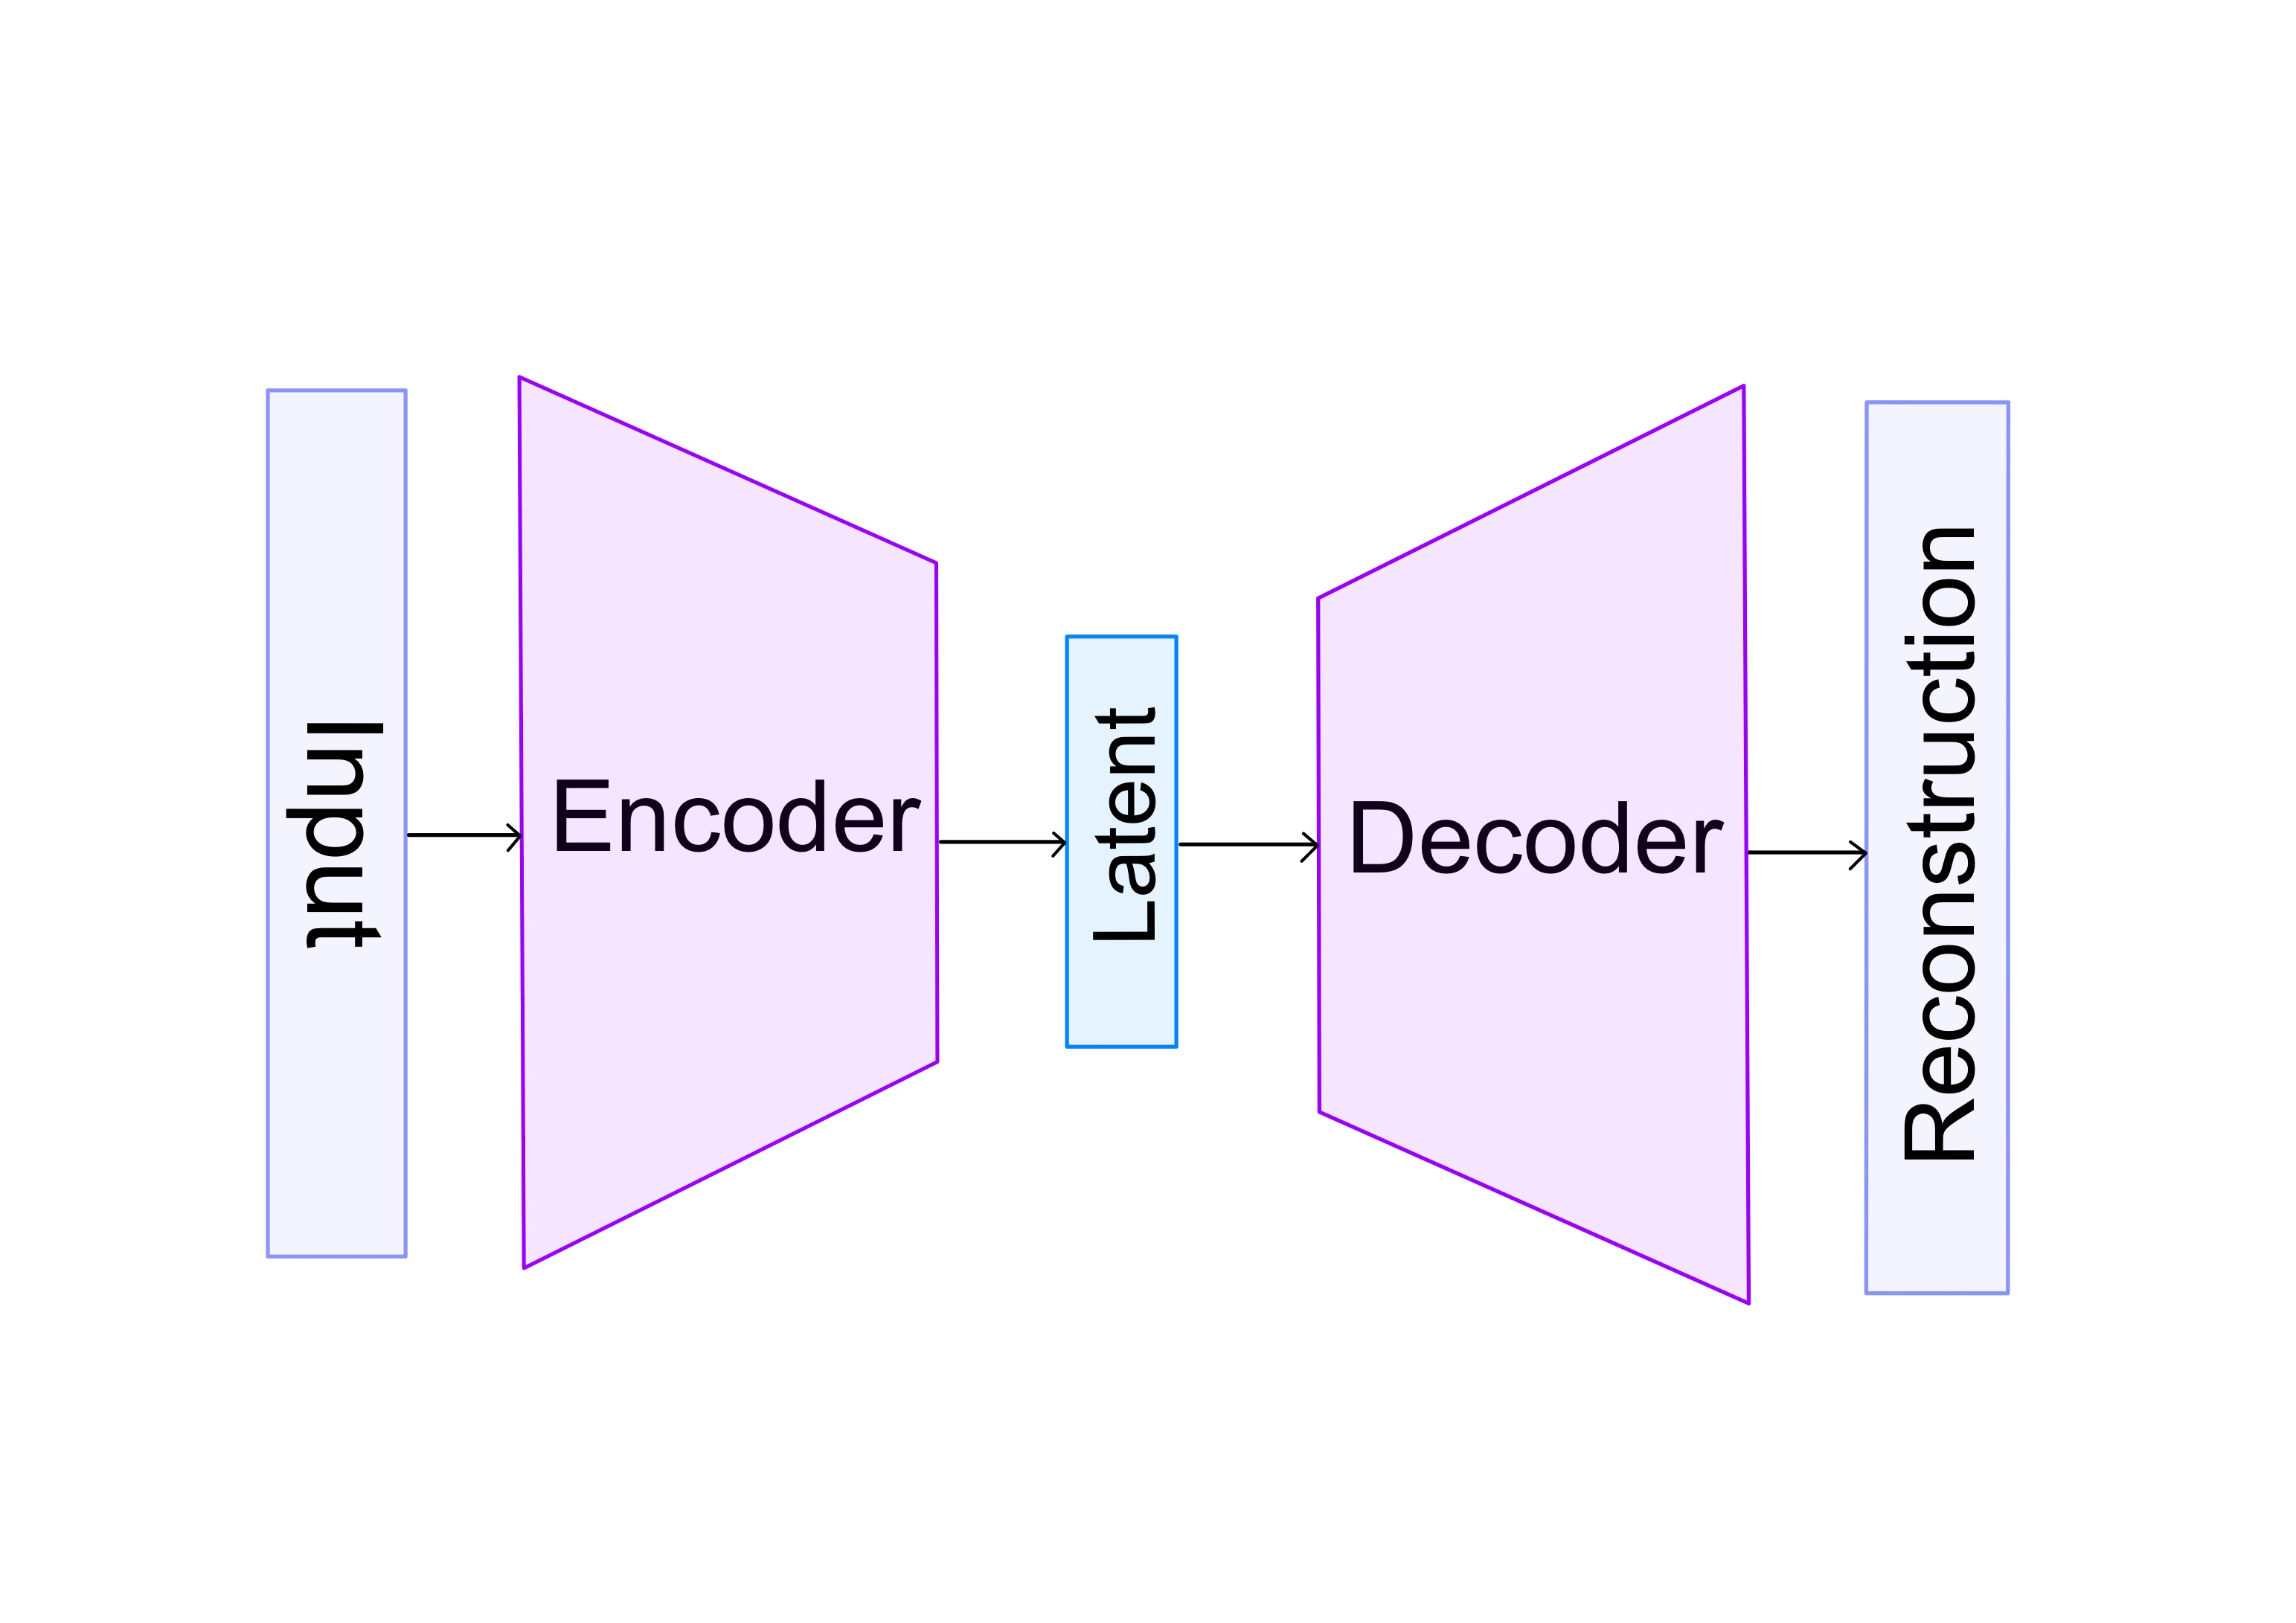
\includegraphics[width=0.6\textwidth]{AE.jpg}  % Change 'image.png' to the name of your image file
    \caption{Auto-Encoder Architecture}
    \label{fig:AutoencoderArchitecture}
\end{figure}\\\\
This notion of a vectorized latent embedding which captures core information raises interesting questions. Can we take two data samples, get their latent embeddings, linearly interpolate their embeddings and then run this interpolation through the decoder to get a sample which somehow combines the core features of both samples? Can we somehow sample from the latent space to generate wholly novel samples which come from the same distribution as our original data? If we were attempt to do either of these things using a standard Auto-Encoder we would often find that an issue is the lack of regularity of the latent space. What we mean by this is that there is nothing in the architecture of an Auto-Encoder which, for instance, ensures that the latent space surrounding a particular latent embedding will produce samples ``similar" to that latent embedding, or that there is any inherent regular distributional structure to the latent space. Although the Auto-Encoder often cluster similar inputs to similar latent embeddings naturally in order for efficient reproductions, the lack of an explicit enforcing of latent space regularity leads to the issue of i) not having a distribution to sample from and ii) not being able to ensure that the latent space surrounding a specific embedding holds ``similar" embeddings, ie: a lack of regularity. These issues are addressed in the modified VAE architecture as described below.

\subsubsection{General Description}
Variational Auto-Encoders (VAEs) are a class of generative neural networks which consist of an encoder and decoder. The encoder maps the input data into a latent space, typically of lower dimension than that of the input, and the decoder maps latent-embeddings back into the ``real-world" space. The encoder can be interpreted as applying a non-linear dimensionality reduction to the input data. The aim of the encoder is to learn a useful latent-representation of the data, where core/informative features are captured in the dimensions of the latent space. A key feature of VAEs over their cousin the Auto-Encoder is that VAEs attempt to force the latent space to be more regular. This can be achieved by penalising the estimated latent space to ensure that it is closer to some prior distribution of our choice. This allows us to sample from the continuous prior after training and consequently pass our samples through the decoder to generate novel data samples that in theory come from the same distribution as our original data.

\subsubsection{Formal Description}
The formal description that follows is closely based on the work of (\cite{kingma2019introduction}). \\\\Let $\mathbf{x}$ be a vector representing the $k$-dimensional data whose joint distribution we would like to model. Let $p^{*}(\mathbf{x})$ denote the true distribution of $X$. Our goal is to approximate $p^{*}(\mathbf{x})$ with a parameterised model $p_{\boldsymbol{\theta}}(\mathbf{x})$. In other words, we wish to find parameters $\boldsymbol{\theta}$ such that $$\mathbf{x} \sim p^{*}(\mathbf{x}) \approx p_{\boldsymbol{\theta}}(\mathbf{x}).$$ It holds that we would like the family of models possible under our parameterisation to be highly flexible, as we do not know how complex the true distribution $p^{*}(\mathbf{x})$ may be. Neural Networks give such a family of models.
\\\\
We can then introduce the notion of $\textit{latent variables}$, denoted $\mathbf{z}$, also known as unobservable variables due to the fact that they are not found explicitly in our dataset. Although they are unobserved, they appear in our model through $\mathbf{x}$'s conditional dependence on them. Their distribution, $p(\mathbf{z})$, is known as the prior distribution over $\mathbf{z}$. Via the law of total probability and Bayes' formula we get 
\numberwithin{equation}{section}

\begin{align}
\label{bayesformula}
p_{\boldsymbol{\theta}}(\mathbf{x}) &= \int p_{\boldsymbol{\theta}}(\mathbf{x}, \mathbf{z}) \, d\mathbf{z} \\
\end{align}
and
\begin{align}
\label{LOTP}
p_{\boldsymbol{\theta}}(\mathbf{x}, \mathbf{z}) &= p_{\boldsymbol{\theta}}(\mathbf{x}|\mathbf{z})p(\mathbf{z}).
\end{align}
\\
When such models are parameterised using deep neural networks they are termed \textit{deep latent variable models} (DLVM). A benefit of DVLM's is that even when each factor in \ref{LOTP} (namely the conditional and prior distributions) are relatively simple (for example, Gaussian), the resulting marginal $p_{\boldsymbol{\theta}}(\mathbf{x})$ can be very complex as a result of \ref{bayesformula}. This is what makes DVLM's attractive when approximating possibly complex distributions.
\\\\
When attempting to maximise the likelihood of DVLM's we run into the issue that the marginal $p_{\boldsymbol{\mathbf{\theta}}}(\mathbf{x})$ is typically intractable due to the integral in \ref{bayesformula} either not having an analytic solution, or being computationally intractable under estimation. As a consequence we cannot differentiate with regards to (w.r.t) the parameters so as to be able to maximise the likelihood. This intractability also carries over to the posterior distribution $p_{\boldsymbol{\theta}}(\mathbf{z}|\mathbf{x})$ via 
\begin{align}
\label{Bayes2}
p_{\boldsymbol{\theta}}(\mathbf{z}|\mathbf{x}) &= \frac{p_{\boldsymbol{\theta}}(\mathbf{x}, \mathbf{z})}{p_{\boldsymbol{\theta}}(\mathbf{x})}.
\end{align}
\\\\
In order to address these issues of intractability we introduce a parameterised, approximate posterior

\begin{align}
q_{\boldsymbol{\phi}}(\mathbf{z}|\mathbf{x}) \approx p_{\boldsymbol{\theta}}(\mathbf{z}|\mathbf{x})
\end{align}

\subsubsection{KL-Divergence}
Although there are many methods to penalise the ``distance" between two distributions, historically Kullback-Leibler(KL) divergence has been used in the context of VAEs in order to get such a measure of ``distance", motivated below in the derivation regarding the evidence lower bound. It must be noted that KL divergence is not a true metric in the sense that it fails to be symmetric.\\\\
Formally, KL-divergence is the expected difference in information of one probability distribution, $q$ to another distribution $p$, where the expectation is taken under $q$. Mathematically it is defined as
\begin{align}
D_{KL}(q||p) =\mathbb{E}_{q(\mathbf{x})}\left[\text{log}\left(\frac{q(\mathbf{x})}{p(\mathbf{x})}\right)\right]
\end{align}
The definition stems from information theory, and can be informally interpreted as how surprised one is from using $p$ as a distribution to describe the process in question when the true distribution of the process is $q$ (\cite{KLWikipedia2024}).
\\\\
Recall Jensen's inequality, namely that if $(\Omega, \mathcal{F}, \mu$) is a measure space, $f:\Omega \rightarrow \mathbb{R}$ a measurable function, and $\varphi: \mathbb{R} \rightarrow \mathbb{R}$ a convex function, then
\begin{align}
\varphi \left ( \int_{\Omega} f d\mu\right) \leq \int_{\Omega} \varphi (f) d\mu.
\end{align}
If $\varphi$ is a strictly convex function and $f$ is non-degenerative (i.e.: non-constant) on a set $A$ with $\mu(A)>0$, then the inequality is strict.

\begin{claim}{}
KL divergence is non-negative.
\end{claim}

\begin{proof}
We have that $-log: \mathbb{R} \rightarrow \mathbb{R}$ is a convex function, hence by letting $f = \frac{p(\mathbf{x})}{q(\mathbf{x})}$ we get
\begin{align}
D_{KL}(q||p) &=\mathbb{E}_{q(\mathbf{x})}\left[-\text{log}\left(\frac{p(\mathbf{x})}{q(\mathbf{x})}\right)\right] \\
\label{KLinequality}
&\geq - \text{log} \int_{\mathbb{R}} q(\mathbf{x}) \frac{p(\mathbf{x})}{q(\mathbf{x})} dx \\
& = -\text{log} \int_{\mathbb{R}} p(\mathbf{x}) dx \\
& = - \text{log}(1) = 0
\end{align} 
\end{proof}

\begin{claim}
 $D_{KL}(q||p) = 0$ if and only if (iff) $p=q \quad \mathbb{P}_{q(\mathbf{x})}$ almost everywhere (a.e).
\end{claim}

\begin{proof}
$(\Rightarrow)$
Suppose that $D_{KL}(q||p) = 0$, then since -log is a strictly convex function, we can only have equality in \ref{KLinequality} if $-\text{log}\frac{p(\mathbf{x})}{q(\mathbf{x})}$ is degenerative everywhere except on a set of measure zero, ie: 
\begin{align*}
D_{KL}(q||p) &= 0\\
\Rightarrow
p(\mathbf{x}) &= q(\mathbf{x}) \qquad \mathbb{P}_{q(\mathbf{x})} \quad a.e.
\end{align*}
$(\Leftarrow)$\\ Suppose that $p=q \quad \mathbb{P}_{q(\mathbf{x})}$ a.e, then 
\begin{align*}
D_{KL}(q||p) &= \mathbb{E}_{q(\mathbf{x})}\text{log}\left(\frac{q(\mathbf{x})}{p(\mathbf{x})}\right)\\
&=\int_{\Omega} {log}\left(\frac{q(\mathbf{x})}{p(\mathbf{x})}\right) \mathbb{I}_{\{q(\mathbf{x})=p(\mathbf{x})\}} d \mathbb{P}_{q(\mathbf{x})}\\
&=\int_{\{q(\mathbf{x})=p(\mathbf{x})\}}(\text{log}(1)) d \mathbb{P}_{q(\mathbf{x})} \\
&= 0.\\
\end{align*}
\end{proof}
\subsubsection{Evidence lower bound(ELBO)}
As with many problems of estimating the true distribution of a process, $p(\mathbf{x})$, we wish to maximise the likelihood of our data being observed under our approximate, parameterised distribution, $p_{\boldsymbol{\theta}}(\mathbf{x})$. The evidence/variational lower bound provides a lower bound for the log-likelihood of our estimate. Let $q_{\boldsymbol{\phi}}(\mathbf{z}|\mathbf{x})$ denote our inference model/decoder, $p_{\boldsymbol{\theta}}(\mathbf{z}|\mathbf{x})$ be the parameterised but intractable posterior and let $p_{\boldsymbol{\theta}}(\mathbf{x})$ the marginal distribution of $\mathbf{X}$ under our parameterisation.\\ We have that 
\begin{align}
\text{log}p_{\boldsymbol{\theta}}(\mathbf{x})
&= \mathbb{E}_{q_{\boldsymbol{\phi}}(\mathbf{z}|\mathbf{x})}\left[\text{log}p_{\boldsymbol{\theta}}(\mathbf{x})\right]\\
&=\mathbb{E}_{q_{\boldsymbol{\phi}}(\mathbf{z}|\mathbf{x})}\left[\text{log}\left(\frac{p_{\boldsymbol{\theta}}(\mathbf{x}, \mathbf{z})}{p_{\boldsymbol{\theta}}(\mathbf{z}|\mathbf{x})}\right)\right]\\
&=\mathbb{E}_{q_{\boldsymbol{\phi}}(\mathbf{z}|\mathbf{x})}\left[\text{log}\left(\frac{p_{\boldsymbol{\theta}}(\mathbf{x}, \mathbf{z})}{q_{\boldsymbol{\phi}}(\mathbf{z}|\mathbf{x})}\frac{q_{\boldsymbol{\phi}}(\mathbf{z}|\mathbf{x})}{p_{\boldsymbol{\theta}}(\mathbf{z}|\mathbf{x})}\right)\right]\\
&=\mathbb{E}_{q_{\boldsymbol{\phi}}(\mathbf{z}|\mathbf{x})}\left[\text{log}\left(\frac{p_{\boldsymbol{\theta}}(\mathbf{x}, \mathbf{z})}{q_{\boldsymbol{\phi}}(\mathbf{z}|\mathbf{x})}\right)\right]+\mathbb{E}_{q_{\boldsymbol{\phi}}(\mathbf{z}|\mathbf{x})}\left[\text{log}\left(\frac{q_{\boldsymbol{\phi}}(\mathbf{z}|\mathbf{x})}{p_{\boldsymbol{\theta}}(\mathbf{z}|\mathbf{x})}\right)\right]\\
&=\mathcal{L}_{\boldsymbol{\theta}, \boldsymbol{\phi}}(\mathbf{x})+D_{KL}(q_{\boldsymbol{\phi}}(\mathbf{z}|\mathbf{x})||p_{\boldsymbol{\theta}}(\mathbf{z}|\mathbf{x}))
\end{align}
\\
The first term is called the variational/evidence lower bound (ELBO), denoted $\mathcal{L}_{\boldsymbol{\theta}, \boldsymbol{\phi}}(\mathbf{x})$, and the second term is the KL-divergence between $q_{\boldsymbol{\phi}}(\mathbf{z}|\mathbf{x})$ and $p_{\boldsymbol{\theta}}(\mathbf{z}|\mathbf{x})$, denoted $D_{KL}(q_{\boldsymbol{\phi}}(\mathbf{z}|\mathbf{x})||p_{\boldsymbol{\theta}}(\mathbf{z}|\mathbf{x})).$\\\\
Since the KL-divergence is always non-negative, we see that the evidence lower bound is indeed a lower bound for the log-likelihood, i.e.:
$$\text{log}p_{\boldsymbol{\theta}}(\mathbf{x}) \geq \mathcal{L}_{\boldsymbol{\theta}, \boldsymbol{\phi}}(\mathbf{x}).$$
Rearranging gives $$\mathcal{L}_{\boldsymbol{\theta}, \boldsymbol{\phi}}(\mathbf{x})=\text{log}p_{\boldsymbol{\theta}}(\mathbf{x})-D_{KL}(q_{\boldsymbol{\phi}}(\mathbf{z}|\mathbf{x})||p_{\boldsymbol{\theta}}(\mathbf{z}|\mathbf{x}))$$
which has a very satisfying interpretation. We see that by maximising the ELBO, we not only approximately maximise the marginal log-likelihood of $\mathbf{X}$, but also minimise the KL divergence between the true and approximated posterior distributions.\\\\
Manipulating the ELBO we find:
\begin{align}
\mathcal{L}_{\boldsymbol{\theta}, \boldsymbol{\phi}}(\mathbf{x})
&=\mathbb{E}_{q_{\boldsymbol{\phi}}(\mathbf{z}|\mathbf{x})}\left[\text{log}\left(\frac{p_{\boldsymbol{\theta}}(\mathbf{x}| \mathbf{z})p(\mathbf{z})}{q_{\boldsymbol{\phi}}(\mathbf{z}|\mathbf{x})}\right)\right]\\
&=\mathbb{E}_{q_{\boldsymbol{\phi}}(\mathbf{z}|\mathbf{x})}\left[\text{log}\left(p_{\boldsymbol{\theta}}(\mathbf{x}| \mathbf{z})\right)\right]-\mathbb{E}_{q_{\boldsymbol{\phi}}(\mathbf{z}|\mathbf{x})}\left[\text{log}\left(\frac{{q_{\boldsymbol{\phi}}(\mathbf{z}|\mathbf{x})}}{p_{\boldsymbol{\theta}}(\mathbf{z})}\right)\right]\\
\label{elboexpansion1}
&=\mathbb{E}_{q_{\boldsymbol{\phi}}(\mathbf{z}|\mathbf{x})}\left[\text{log}\left(p_{\boldsymbol{\theta}}(\mathbf{x}| \mathbf{z})\right)\right]-D_{KL}(q_{\boldsymbol{\phi}}(\mathbf{z}|\mathbf{x})||p_{\boldsymbol{\theta}}(\mathbf{z}))\\
&=\text{Reconstruction Loss} - \text{KL Divergence}
\end{align}
The first term in \ref{elboexpansion1} is termed the \textit{reconstruction} loss and the second is the KL divergence between our approximate posterior distribution and our prior distribution.

\subsubsection{Deriving the loss function}
We now derive an explicit form for the loss function of our neural network, which in our case is the negative ELBO. In order to do this, we must decide on forms for both the prior, posterior and decoder distributions. 
The most common case, and indeed what we used when implementing the VAE, is to choose the prior and posterior to be Gaussian distributions with diagonal covariance matrices:
\begin{align}
q_{\boldsymbol{\phi}}(\mathbf{z}|\mathbf{x}) &\sim \mathcal{N}\left(\mathbf{x}, \boldsymbol{\mu}(\mathbf{x}), \text{diag}\left(\boldsymbol{\sigma}^{2}(\mathbf{x})\right)\right)
\end{align}
and
\begin{align}
p(\mathbf{z}) &\sim \mathcal{N}(\mathbf{0}, \mathbb{I})
\end{align}
where
\begin{align}
    \left(\boldsymbol{\mu}(\mathbf{x}), \text{log}\left(\boldsymbol{\sigma}^{2}(\mathbf{x})\right)\right) = \text{EncoderNeuralNetwork}_{\boldsymbol{\phi}}(\mathbf{x})
\end{align}
Recall that the distribution function for a $d$-dimensional multivariate gaussian random variable $\mathbf{Y}$ is of the form 
\begin{align}
    p_\mathbf{Y}(\mathbf{y})=\left((2\pi)^{d}|\boldsymbol{\Sigma}|\right)^{-\frac{1}{2}} \text{exp}\left[(\mathbf{y}-\boldsymbol{\mu})^{T}\boldsymbol{\Sigma}^{-1}(\mathbf{y}-\boldsymbol{\mu})\right]
\end{align}
where $\boldsymbol{\Sigma}$ is the covariance matrix of $\mathbf{Y}$.\\\\
Thus the densities for the prior and posterior are 
\begin{align}
    p(\textbf{z}) = (2\pi)^{-\frac{d}{2}}\text{exp}\left(-\frac{1}{2}\sum_{i=1}^{d} (z_{i})^2\right)
\end{align}
and 
\begin{align}
    q_{\boldsymbol{\phi}}(\mathbf{z}|\mathbf{x})=\left((2\pi)^{d}|\boldsymbol{\Sigma}|\right)^{-\frac{1}{2}}\text{exp}\left(-\frac{1}{2}\sum_{i=1}^{d}\left(\frac{z_i-\mu_i}{\sigma_i}\right)^2\right)
\end{align}
Focusing on the KL Divergence term in the ELBO \ref{elboexpansion1} and subbing in the chosen densities for the prior and posterior gives:
\begin{align}
    &D_{KL}(q_{\boldsymbol{\phi}}(\mathbf{z}|\mathbf{x})||p_{\boldsymbol{\theta}}(\mathbf{z}))\\ 
    &= \mathbb{E}_{q_{\boldsymbol{\phi}}(\mathbf{z}|\mathbf{x})}\left[\text{log}\left(\frac{{q_{\boldsymbol{\phi}}(\mathbf{z}|\mathbf{x})}}{p_{\boldsymbol{\theta}}(\mathbf{z})}\right)\right]\\
    &=\mathbb{E}_{q_{\boldsymbol{\phi}}(\mathbf{z}|\mathbf{x})}\left[\text{log}q_{\boldsymbol{\phi}}(\mathbf{z}|\mathbf{x}) - \text{log}p(\textbf{z})\right]\\
    &=\mathbb{E}_{q_{\boldsymbol{\phi}}(\mathbf{z}|\mathbf{x})}\left[-\frac{1}{2}\left(\text{log}(2\pi)^d+\text{log}|\boldsymbol{\Sigma}|-\sum_{i=1}^{d}\left(\frac{z_i-\mu^i}{\sigma_i}\right)^2+\text{log}(2\pi)^d+\sum_{i=1}^{d} (z_i)^2\right)\right]\\
    \label{premeansub}
    &=-\frac{1}{2}\left[\text{log}\left(\Pi_{i=1}^d\sigma_i\right) + \sum_{i=1}^d\frac{\mathbb{E}_{q_{\boldsymbol{\phi}}(\mathbf{z}|\mathbf{x})}(z_i-\mu_i)^2}{\sigma_i^2}-\sum_{i=1}^d\mathbb{E}_{q_{\boldsymbol{\phi}}(\mathbf{z}|\mathbf{x})}(z_i^2)\right].
\end{align}\\
Recalling that $\mathbb{E}(z_i^2) = \sigma_i^2-\mu_i^2$ and $\text{Var}(z_i) = \mathbb{E}(z_i-\mu_i)^2$, equation \ref{premeansub} becomes
\begin{align}
    &=-\frac{1}{2}\left[\sum_{i=1}^d\left(\text{log}\sigma_i^2 + 1 -\sigma_i^2-\mu_i^2\right)\right].
\end{align}
\noindent
When dealing with continuous data, the form of the decoder's distribution is assumed to be Gaussian distributed, with mean given by the model's output, and with constant, diagonal covariance structure:
\begin{align}
    p_{\boldsymbol{\theta}}(\mathbf{x}|\mathbf{z}) \sim \mathcal{N}\left(\boldsymbol{\mu}(\mathbf{z}), \boldsymbol{\sigma^2}\mathbb{I}\right)
\end{align} 
where 
$$\boldsymbol{\mu}(\mathbf{z}) = \text{DecoderNeuralNetwork}_{\boldsymbol{\theta}}(\mathbf{z})$$
Let $k$ be the dimensionality of the input $\mathbf{x}$, then the reconstruction error term in \ref{elboexpansion1} becomes:
\begin{align}
\label{reconstruction pre derivative}
    \mathbb{E}_{q_{\boldsymbol{\phi}}(\mathbf{z}|\mathbf{x})}\left[\text{log}\left(p_{\boldsymbol{\theta}}(\mathbf{x}| \mathbf{z})\right)\right] = \mathbb{E}_{q_{\boldsymbol{\phi}}(\mathbf{z}|\mathbf{x})}\left[-\frac{1}{2\sigma^2}\sum_{i=1}^{k}\left(x_i-\mu(z)_i)^2\right)-\frac{k}{2}\text{log}(2\pi\sigma^2)\right] 
\end{align}
Thus the loss function which is the negative ELBO becomes:

\begin{align}
    Loss = \mathbb{E}_{q_{\boldsymbol{\phi}}(\mathbf{z}|\mathbf{x})}\left[\frac{1}{2\sigma^2}\sum_{i=1}^{k}\left(x_i-\mu(z)_i)^2\right)-\frac{k}{2}\text{log}(2\pi\sigma^2)\right] -\frac{1}{2}\left[\sum_{i=1}^d\left(\text{log}\sigma_i^2 + 1 -\sigma_i^2-\mu_i^2\right)\right] 
\end{align}

\subsubsection{Gradient Estimates}
If we wish to use gradient based optimisation techniques such as Stochastic Gradient Descent (SGD) in order to maximise the ELBO (or equivalently, minimise the loss function), we need to be able to find unbiased estimators for the gradient of the ELBO w.r.t both sets of parameters $\boldsymbol{\theta}$ and $\boldsymbol{\phi}$, i.e. we need to get unbiased estimates for:
\begin{align}
\nabla_{\boldsymbol{\theta} \boldsymbol{\phi}}\mathcal{L}_{\boldsymbol{\theta}, \boldsymbol{\phi}}({\mathbf{x}}) &= \nabla_{\boldsymbol{\theta}\boldsymbol{\phi}} \left(\text{Reconstruction Loss}-\text{KL divergence}\right)\\
    &=\nabla_{\boldsymbol{\theta}\boldsymbol{\phi}} \left(\text{Reconstruction Loss}\right)-\nabla_{\boldsymbol{\theta}\boldsymbol{\phi}}\left(\text{KL divergence}\right)\\
\end{align}
Finding gradients for the KL divergence loss term is straightforward as the loss depends only on the outputs of the encoder, which in our case is a differentiable function.\\
Let us now attempt to find the gradient of the Reconstruction Loss.\\\\
We first consider taking the gradient w.r.t $\boldsymbol{\theta}$:
\begin{align}
    \nabla_{\boldsymbol{\theta}} \left(\text{Reconstruction Loss}\right) &=  \nabla_{\boldsymbol{\theta}} \mathbb{E}_{q_{\boldsymbol{\phi}}(\mathbf{z}|\mathbf{x})}\left[\text{log}\left(p_{\boldsymbol{\theta}}(\mathbf{x}| \mathbf{z})\right)\right]\\
    \label{preMC}
    &=\mathbb{E}_{q_{\boldsymbol{\phi}}(\mathbf{z}|\mathbf{x})}\left[\nabla_{\boldsymbol{\theta}}\text{log}\left(p_{\boldsymbol{\theta}}(\mathbf{x}| \mathbf{z})\right)\right]\\
    \label{unbiasedMCestimate}
    &\eqsim \nabla_{\boldsymbol{\theta}}\text{log}\left(p_{\boldsymbol{\theta}}(\mathbf{x}| \mathbf{z})\right)
\end{align}    
where \ref{unbiasedMCestimate} is an unbiased Monte Carlo estimate of \ref{preMC}, gotten by sampling from $\mathbf{z} \sim q_{\boldsymbol{\phi}}(\mathbf{z}|\mathbf{x})$.
\\\\
We however run into issues when attempting to take the derivative w.r.t $\boldsymbol{\phi}$ as we can no longer simply move the derivative inside the integral due to us taking the integral relative to $q_{\boldsymbol{\phi}}(\mathbf{z}|\mathbf{x})$ which depends on $\boldsymbol{\phi}$. A work around is if we can somehow express the stochastic element of $q_{\boldsymbol{\phi}}(\mathbf{z}|\mathbf{x})$ by something independent of $\boldsymbol{\phi}$, allowing us to differentiate through expectation after a change of variables. This approach is famously known as the reparameterisation trick.

\subsubsection{The Reparameterisation Trick}
Suppose we can express  the random variable $\mathbf{z}\sim q_{\boldsymbol{\phi}}(\mathbf{z}|\mathbf{x})$ as the transformation of another random variable $\boldsymbol{\epsilon}$, ie:
\begin{align}
    \mathbf{z} = g(\boldsymbol{\phi}, \mathbf{x}, \boldsymbol{\epsilon})
\end{align}
where $\boldsymbol{\epsilon}$ has some distribution independent of $\boldsymbol{\phi}$ and $ \mathbf{x}$, say  $\boldsymbol{\epsilon} \sim p(\boldsymbol{\epsilon})$, and g is an invertible and differentiable function.\\\\
We can now express expectations under $q_{\boldsymbol{\phi}}(\mathbf{z}|\mathbf{x})$ as being under $p(\boldsymbol{\epsilon})$:
\begin{align}
    \mathbb{E}_{q_{\boldsymbol{\phi}}(\mathbf{z}|\mathbf{x})} f(\mathbf{z}) =  \mathbb{E}_{p(\boldsymbol{\epsilon})} f(\mathbf{z})
\end{align}
and because we are now taking expectation under a distribution independent of $\boldsymbol{\phi}$, the derivative and expecations become commutative as was the case with $\boldsymbol{\theta}$:

\begin{align}
    \nabla_{\boldsymbol{\phi}} \left(\text{Reconstruction Loss}\right) &= \nabla_{\boldsymbol{\phi}} \mathbb{E}_{q_{\boldsymbol{\phi}}(\mathbf{z}|\mathbf{x})}\left[\text{log}\left(p_{\boldsymbol{\theta}}(\mathbf{x}| \mathbf{z})\right)\right]\\
    &=\nabla_{\boldsymbol{\phi}} \mathbb{E}_{p(\boldsymbol{\epsilon})}\left[\text{log}\left(p_{\boldsymbol{\theta}}(\mathbf{x}| \mathbf{z})\right)\right]\\
    \label{pre MC 2}&=\mathbb{E}_{p(\boldsymbol{\epsilon})}\left[\nabla_{\boldsymbol{\theta}}\text{log}\left(p_{\boldsymbol{\theta}}(\mathbf{x}| \mathbf{z})\right)\right]\\
    \label{MC estimate 2}
    &\eqsim \nabla_{\boldsymbol{\theta}}\text{log}\left(p_{\boldsymbol{\theta}}(\mathbf{x}| \mathbf{z})\right)
\end{align}
where line \ref{MC estimate 2} is again a Monte Carlo estimator of \ref{pre MC 2}, however samples of $\mathbf{z}$ are now gotten by randomly sampling $\boldsymbol{\epsilon}$ and applying the transformation $\mathbf{z} = g(\boldsymbol{\phi}, \mathbf{x}, \boldsymbol{\epsilon})$.\\\\
We are thus now able to take the derivates of the ELBO w.r.t both the encoder and decoder's parameters, allowing us to use gradient based optimisation techniques to maximise the ELBO.
\\
\subsubsection{Final Loss}
Revisiting the Reconstruction Loss in \ref{reconstruction pre derivative} and using our new reparameterisation trick to consider the derivative within the expectation, we see that when taking the derivatives w.r.t to $\boldsymbol{\theta}$ and $\boldsymbol{\phi}$, the second term falls away (as it is independent of both the encoder and decoder's parameters), and the constants in front of the summation can be disregarded, meaning we just need to consider terms of the form:
\begin{align}
  -\sum_{i=1}^{n}\left(x_i-\mu(z)_i)^2\right)  
\end{align}
which is the negative of the familiar Mean Squared Error Loss (MSE).\\\\
Thus, by choosing the loss to be the negative ELBO, and using the fact that we will be taking unbiased estimators of the gradient of this loss via sampling under $\epsilon \sim \mathcal{N}(\mathbf{0}, \mathbb{I})$, we arrive at the final loss function for the $j_{th}$ sample $\mathbf{x}_j$:
\begin{align}
    \label{VAEfinallossfunction}
    Loss_j &= \sum_{i=1}^{k}\left(x_{ij}-\mu(z)_{ij}\right)^2 - \frac{1}{2}\sum_{i=1}^d\left(\text{log}\sigma_{ij}^2 + 1 -\sigma_{ij}^2-\mu_i^2\right)\\
    &= \text{MSE}_{\text{loss}} + \text{KL}_{\text{loss}}
\end{align}
\begin{figure}[h]  % [h] places the figure here
    \centering
    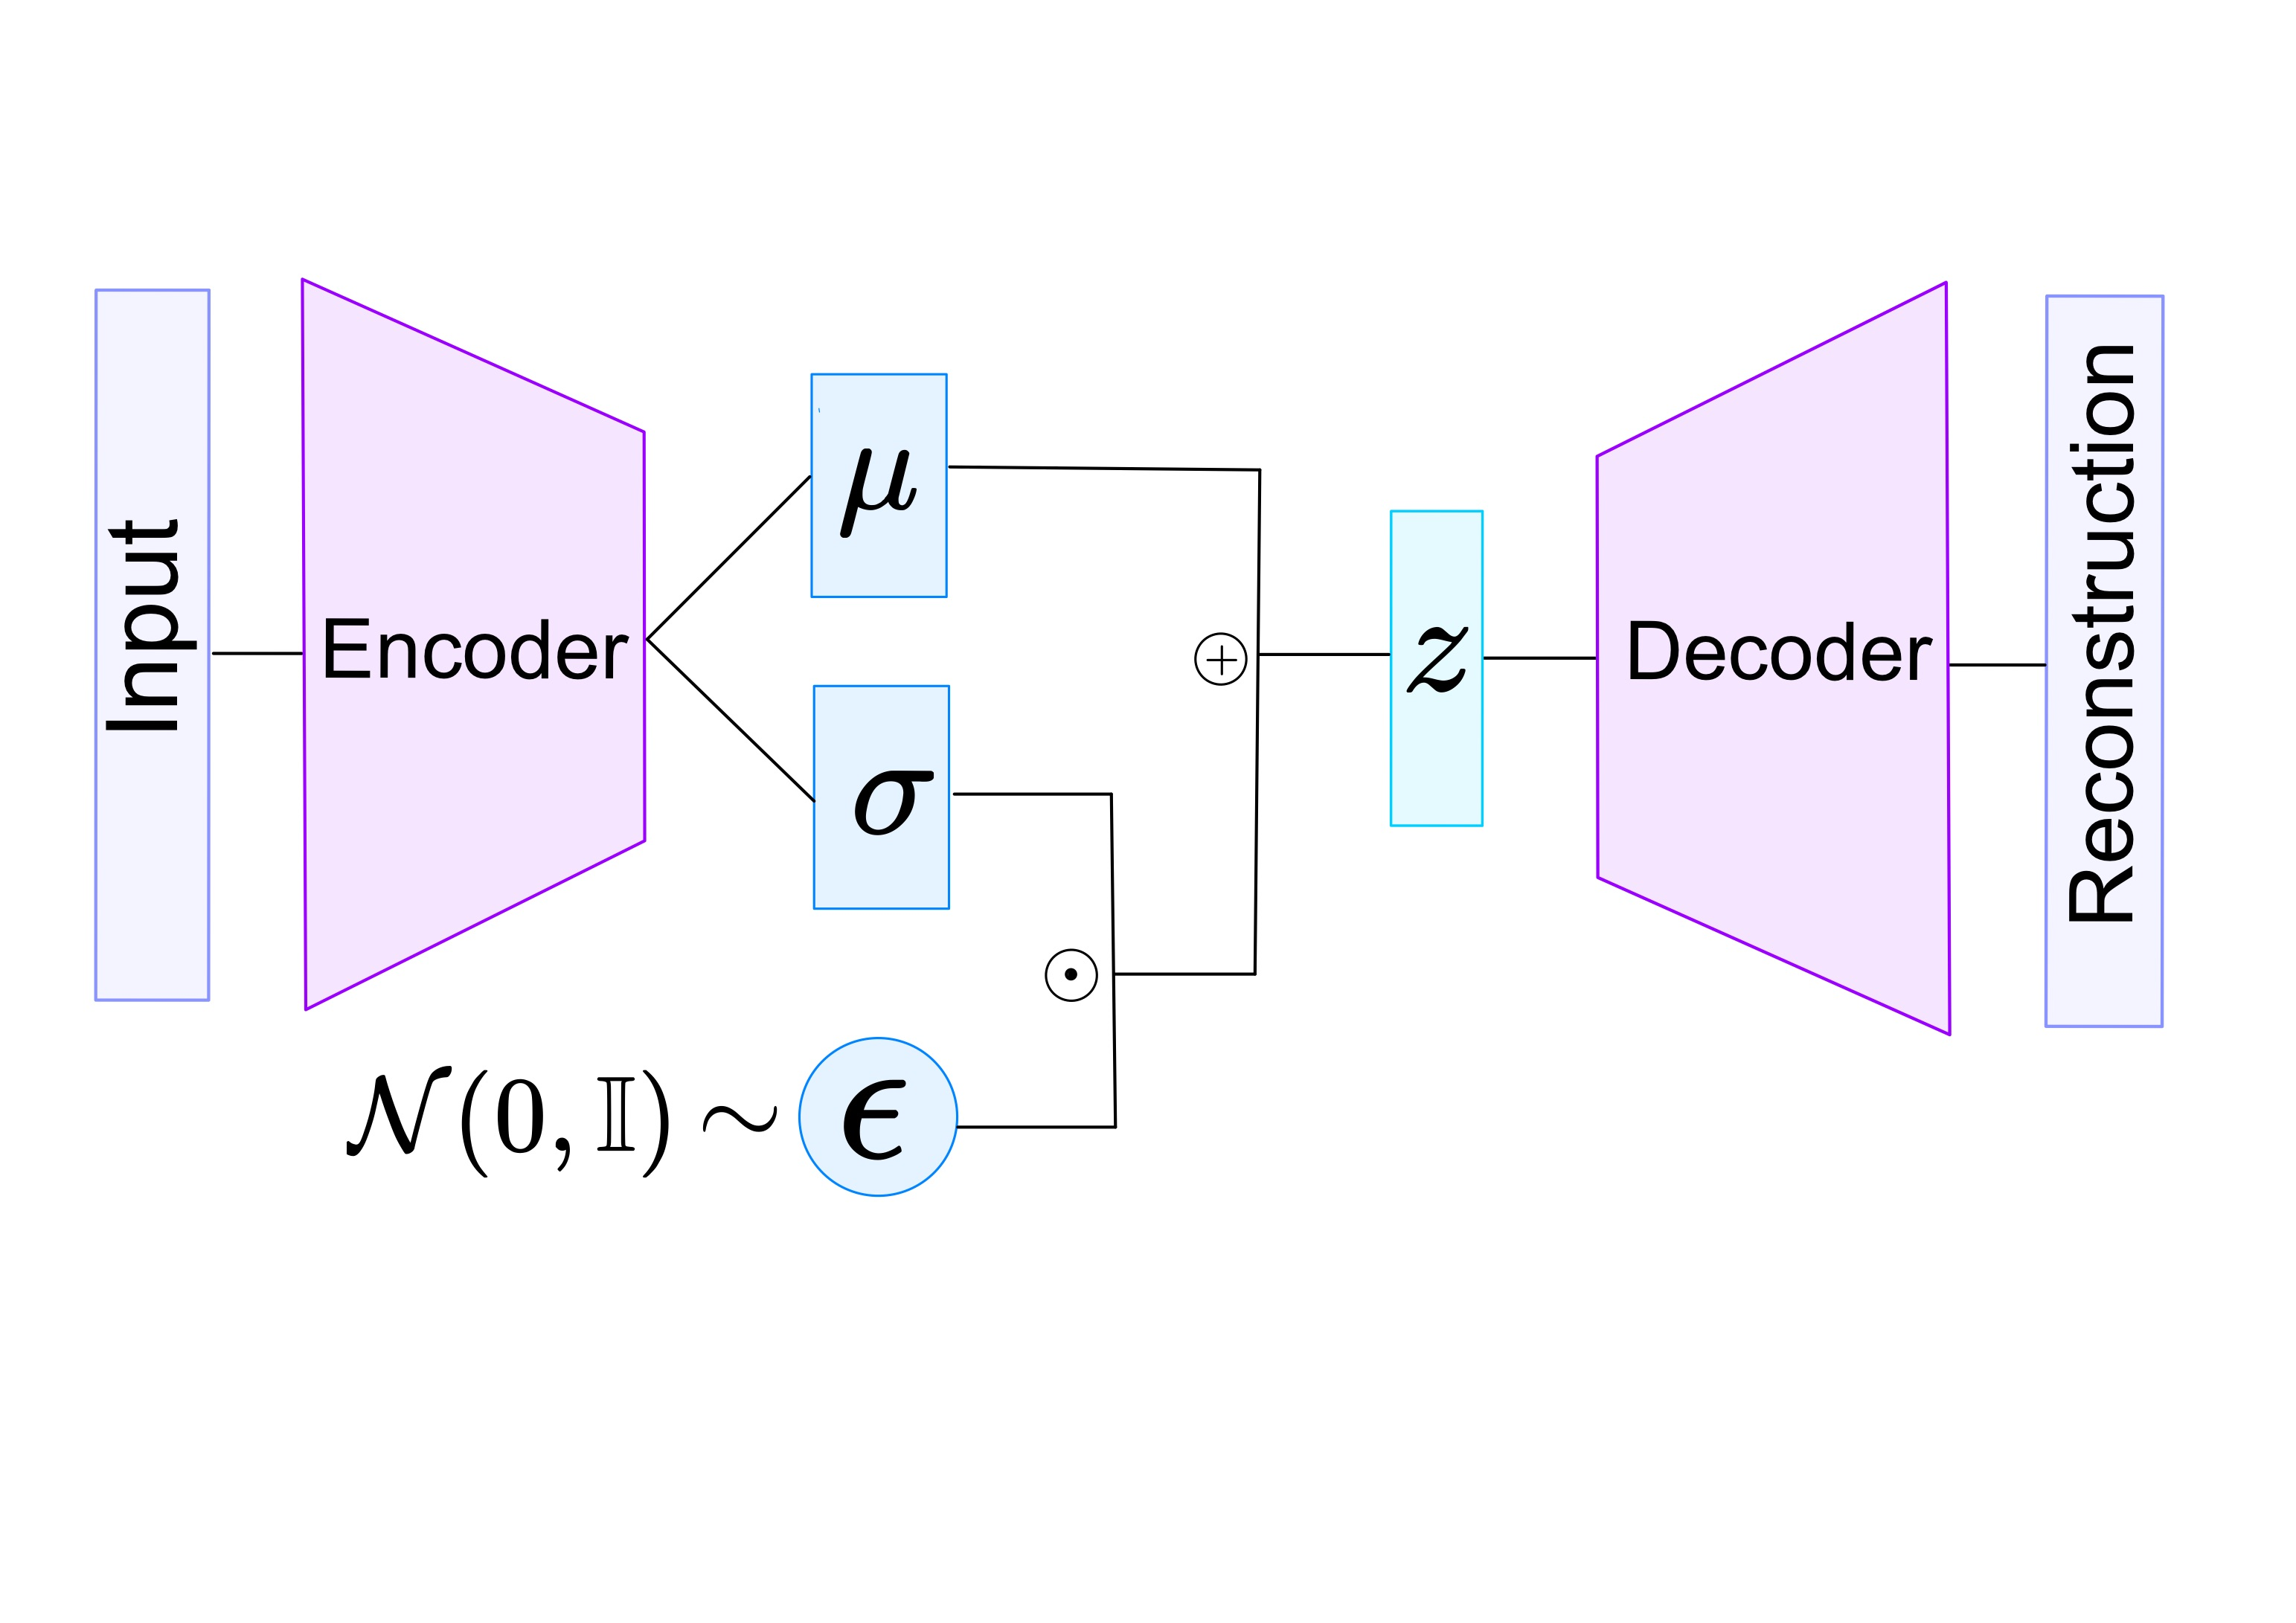
\includegraphics[width=0.6\textwidth]{VAE.jpg}  % Change 'image.png' to the name of your image file
    \caption{Variational Auto-Encoder Architecture.}
    \label{fig:VariationalAutoencoderArchitecture}
\end{figure}\\
\clearpage

\subsubsection{Conditional VAEs}
A modification of the usual VAE architecture was used in this implementation, known as the Conditional VAE (CVAE). A slight modification allows one to append another input to be conditioned on for both the encoder and decoder networks. In our case this has particular relevance in allowing us to condition on the most recent window of time when predicting the next signature, as intuitively the most recent events in time have the most impact on current events. By allowing both the encoder and decoder to take in these conditional inputs, we are also able to condition upon the previously generated signature during market simulation, meaning that generated paths will be more coherent.
\begin{figure}[h]  % [h] places the figure here
    \centering
    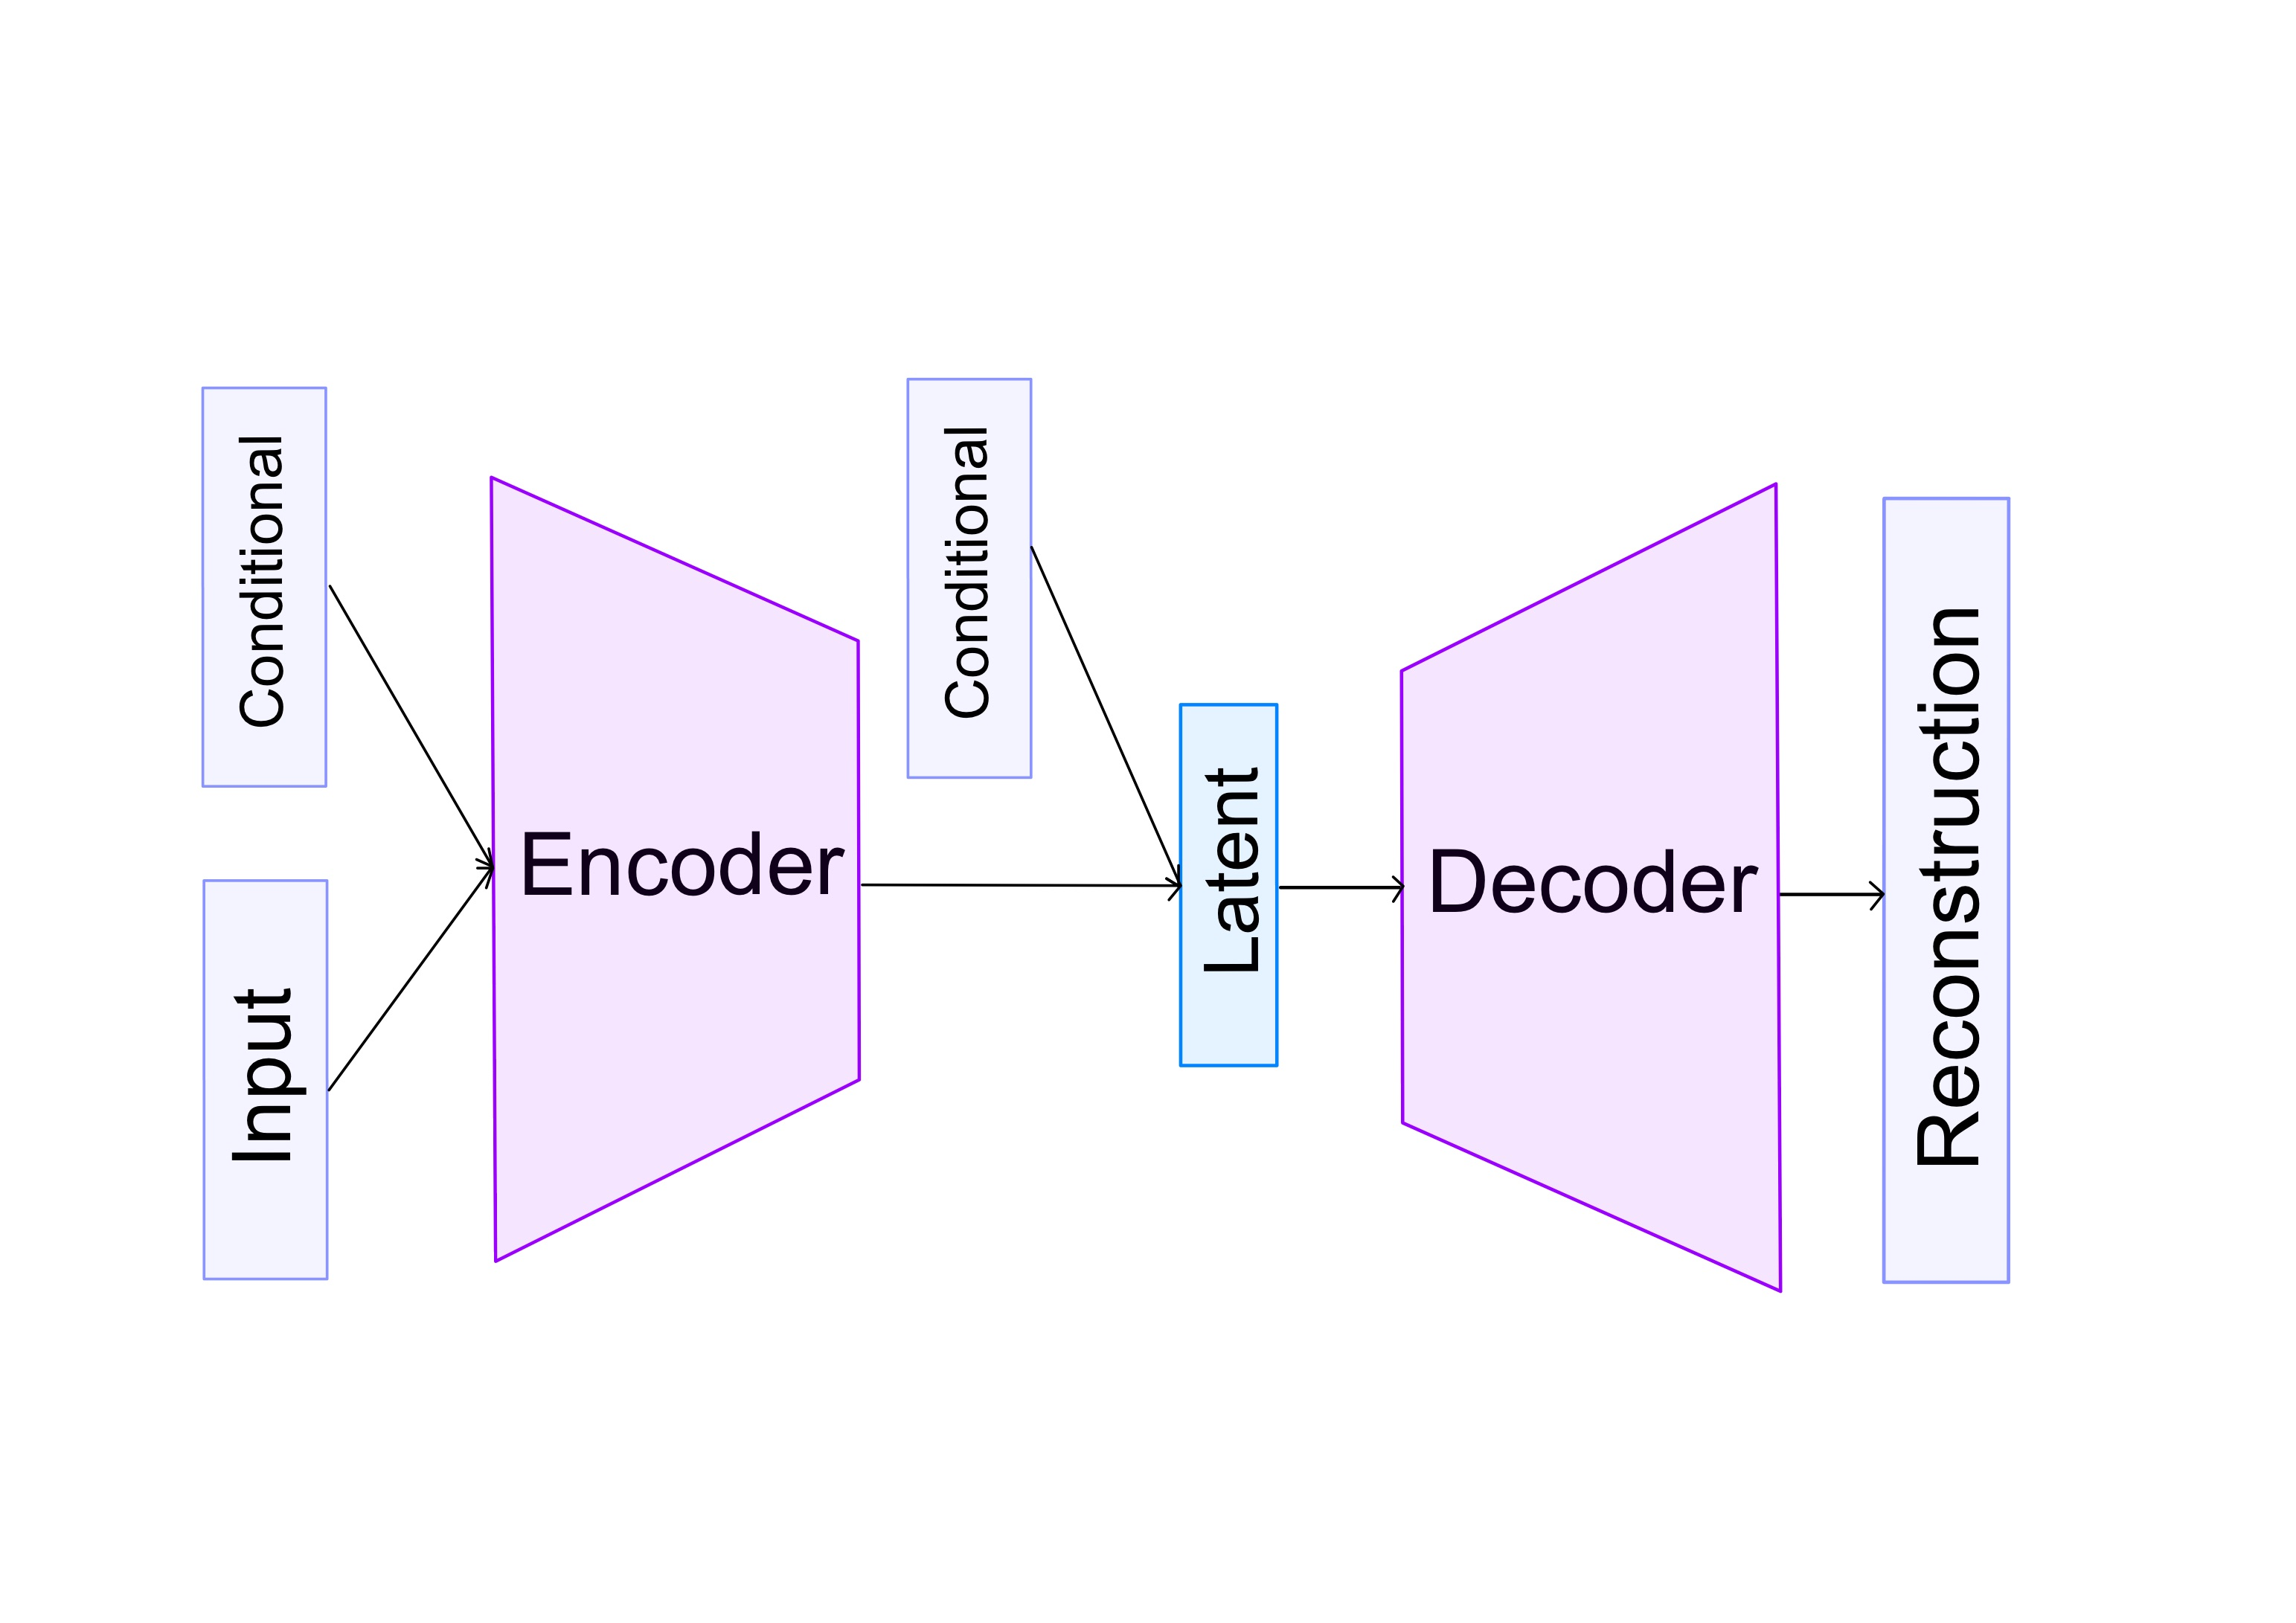
\includegraphics[width=0.6\textwidth]{CVAE.jpg}  % Change 'image.png' to the name of your image file
    \caption{Conditional Variational Auto-Encoder Architecture.}
    \label{fig:AutoencoderArchitecture}
\end{figure}\\

\subsection{Recurrent Neural Networks (RNNs)}
Recurrent Neural Networks are a class of neural network architecture that were created to handle sequential data, where ``memory" of previous inputs would help in the predictive power of the model. A naive approach is to simply put as input to a standard neural network all historical data that one might want the model to consider when making a prediction, however this approach has many drawbacks. Namely, it cannot handle historical data of varying length, and there is no inherent way for the neural network to understand the order in which the data appears (although a simple time index appendage to each data-point is a possible workaround for this). RNNs help address these issues.

\subsubsection{Vanilla RNNs}
Vanilla RNNs hold a memory of past inputs by maintaining a collection of hidden states (one for each layer). At time $t$, the hidden state of layer $1$, $\mathbf{h}_t^1$ is calculated as a function of the previous time step's hidden state at layer $1$, $\mathbf{h}_{t-1}^1$, alongside the latest input vector being considered in the sequence, $\mathbf{x}_t$. At any other layer $l$, the hidden states $\mathbf{h}_t^l$ is similarly defined as a function of $\mathbf{h}_{t-1}^l$ and $\mathbf{h}_t^{l-1}$. The final output of the hidden layer is then a linear transformation of the final hidden state. More specifically, for a network with $L$ hidden layers we have that:
\begin{align}
    &\mathbf{h}_t^1 = \text{tanh}\left(\mathbf{W_h}^1 \mathbf{h}_{t-1}^1 + \mathbf{W_x}^l \mathbf{x}_t + \mathbf{b}^1\right)\\
    &\mathbf{h}_t^l = \text{tanh}\left(\mathbf{W_h}^l \mathbf{h}_{t-1}^l + \mathbf{W_x}^l \mathbf{h}_t^{l-1} + \mathbf{b}^l\right)\\
    &\textbf{\text{output}}_t = \sigma\left(\mathbf{W}_o \mathbf{h}_t^L + \mathbf{b}_o\right)
\end{align}
The major drawback of RNNs is that they suffer from what is know as the issue of vanishing (or exploding) gradients. To explain how this issue arises let's consider some input in our sequence of inputs at time $s$, $\mathbf{x}_s$. The only way for information about $\mathbf{x}_s$ to propogate forward in time is through our hidden states $\mathbf{h}^l$, however, at each new point in our sequence, the previous hidden state is multiplied by the weight matrix $\mathbf{W_h}^l$. Due to regularisation and initialisation, this weight matrix likely has small values in the range $(-1,1)$. What this means is that if we are now at time $t$ with $s<<t$, then the effect of $\mathbf{x}_s$ on our current hidden state $\mathbf{h}_t^l$ (and consequently our output) would become vanishingly small due to successive multiplications by $\mathbf{W_h}^l$. Due to this tendency for inputs in the distant past to have a negligible effect on our current output, Vanilla RNNs are said to have short-term memory.

\subsubsection{Long Short-Term Memory (LSTM) Models}
LSTM models are a form of RNN which were created in order to address the short-term memory issues of Vanilla RNNs, attempting to additionally give them long term-memory.
\\\\
The LSTM differs from standard RNNs in that it has both a cell and hidden state at each layer. The cell state $\mathbf{C}$ helps store and propogate long-term information about sequential inputs, whilst the hidden state $\mathbf{h}$ (as in Vanilla RNNs) can be viewed as a short term memory mechanism.
\\\\
The architecture includes a \textit{forget gate} $\textbf{f}$, an \textit{input gate} $\textbf{i}$, an \textit{output gate} $\textbf{o}$ and a candidate cell state \textit{$\mathbf{\tilde{C}}$}. The forget gate decides how much of the previous time step's cell state to remember. The input gate governs how much of the candidate cell state will be included in the current cell state. The output gate determines which parts of the the cell state are used for the hidden state (and consequently the output). The candidate cell state governs which new information to incorporate into the long-term memory. More formally, we have that 
\begin{align}
    &\mathbf{f}_t = \sigma\left(\mathbf{W}_{fh} \mathbf{h}_{t-1} + \mathbf{W}_{fx} \mathbf{x}_t + \mathbf{b}_{f}\right)\\
    &\mathbf{i}_t = \sigma\left(\mathbf{W}_{ih} \mathbf{h}_{t-1} + \mathbf{W}_{ix} \mathbf{x}_t + \mathbf{b}_{i}\right)\\
    &\mathbf{\tilde{C}}_t = \text{tanh}\left(\mathbf{W}_{Ch}\mathbf{h}_{t-1} + \mathbf{W}_{Cx} \mathbf{x}_t + \mathbf{b}_C\right) 
\end{align}
i.e. the forget gate, input gate and candidate cell state are all simply functions of the previous hidden state, and the current input.
\\\\
The cell state, output gate and hidden state are defined as follows:
\begin{align}
    &\mathbf{C}_t = \mathbf{f}_t \odot \mathbf{C}_{t-1} + \mathbf{i}_t \odot \mathbf{\tilde{C}_t}\\
    &\mathbf{o}_t = \sigma\left(\mathbf{W}_{oh} \mathbf{h}_{t-1} + \mathbf{W}_{ox} \mathbf{x}_t + \mathbf{b}_{o}\right)\\
    &\mathbf{h}_t = \mathbf{o}_t \odot \text{tanh}(\mathbf{C}_t)\\
    &\textbf{\text{output}}_t = \sigma\left(\mathbf{W} \mathbf{h}_t + \mathbf{b}\right)
\end{align}
where $\odot$ denotes the element-wise multiplication of two vectors.
\\\\
These definitions extent naturally to the multilayer case by simply replacing all $\mathbf{x}_t$'s with the previous layer's hidden state output when not considering the very first layer, as was the case for the Vanilla RNN. For example: 
\begin{align}
    \mathbf{f}_t^l = \sigma\left(\mathbf{W}_{fh}^l \mathbf{h}_{t-1}^l + \mathbf{W}_{fx}^l \mathbf{h}_t^{l-1} + \mathbf{b}_{f}^l\right)
\end{align}
We see that the cell state is an element-wise combination of the previous cell state and the new candidate cell state. In this way, we have removed the repeated multiplication by a weight matrix, meaning that long term information does not necessarily get degraded over time. 

\begin{figure}[h]  % [h] places the figure here
    \centering
    
\includegraphics[width=0.7\textwidth]{LSTM_architecture.jpg}  % Change 'image.png' to the name of your image file
    \caption{single-layer LSTM Architecture}
    \label{fig:LSTMArchitecture}
\end{figure}\\\\

\subsection{Deep Hedging}
With the proliferation of the use of DNNs to tackle previously unsolved problems, the issue of whether or not DNNs can be effectively used for the problem of hedging financial instruments has been explored greatly. Thus, it stands that the research questions asked in this paper are not wholly original, although as far as we are aware no one has ever done this specific implementation of joint-distribution generation via path signatures to train a best-of basket option hedger.\\\\
The paper of \cite{buehler2019deep} showed that recurrent neural networks can effectively reproduce the hedging results of more traditional models when no transaction costs are considered, and could in fact provide better performance when transaction costs are included.\\\\
The work of \cite{stangroom2023deephedging} expanded upon these findings, showing that the more specific LSTM architecture further improves hedging capabilities, and that the use of pseudo-real path generation offers a performance boost to DNN hedgers.

\newpage
\section{Methodology}
\subsubsection{Reproducibility}
Throughout all of our code and for all libraries which use pseudo-random number generation, we fixed our seeds to the value of $2024$ should the reader like to reproduce our results.\\\\
All the code written for the project can be found in the GitHub repository https://github.com/NickBossi/Hedging-Honours-Project (\cite{bossi2024hedging}).
\subsection{Path Generation}
\subsubsection{Data Collection}
The two historical stock prices of Apple (\cite{yahoo_finance_apple}) and Microsoft (\cite{yahoo_finance_microsoft}) were downloaed from the Yahoo! finance website and the Opening price of the stocks for the period of 26/06/2020-17/06/2024, corresponding to 1000 days of historical price data.

\subsubsection{Data Pre-Processing}
The 1000 days of historical price data was divided into 200 subpaths of dimension 2 (for the two stocks), each of length 5 days.
The log-signature of each of these 200  (5 x 2) subpaths were then taken using the iisignature package \cite{iisignature}, each producing a log-signature of dimension 14. After this, the data was normalised to be in the interval $[0,1]$ using sklearn MinMaxScaler, which linearly scales down features to be in a fixed range, thus not reducing the effect of outliers. The parameters for the scaler were stored so that they could eventually be used to denormalise the generated samples.
These normalised log-signatures were then used as input to train the CVAE.

\subsubsection{CVAE}
The hyperparameters for the CVAE we informed by those used in \cite{buehler2020data}, with adjustments being made to both the KL weighting and number of nodes in the hidden layers in order to accommodate the difference in data (the simulation of two paths, instead of one). The CVAE followed a simple design with three hidden layers: one for the encoder, one for the latent space and one for decoder.\\
The table below summarises the hyperparameters used:
\begin{table}[h]
\centering
\begin{tabular}{|c|c|}
\hline
\textbf{Hyperparameter} & \textbf{Value} \\
\hline
Kl weighting & 0.003 \\
latent dimension & 8 \\
width of hidden layers & 100 \\
hidden layer activations & LeakyReLU\\
LeakyReLU negative slope & 0.3\\
output activation & sigmoid \\
batch size & 16 \\
learning rate & 0.0003 \\
number of epochs & 20 000 \\
\hline
\end{tabular}
\caption{Hyperparameter Configuration of VAE}
\label{tab:hyperparams}
\end{table}
\\\\
\subsubsection{Loss function}
With the pre-determined KL weighting of 0.003, the loss function for the VAE per training example becomes $$Loss = 0.997 \times \text{MSE} + 0.003 \times \text{KL}_{\text{loss}}$$ where the MSE and $\text{KL}_{\text{loss}}$ terms are calculated as in \ref{VAEfinallossfunction}.
\subsubsection{Generation}

After training, the marginal distributions of the latent embeddings of the training data were plotted, visualised~\ref{fig:latentspaces} below:
\begin{figure}[h]  % [h] places the figure here
    \centering
    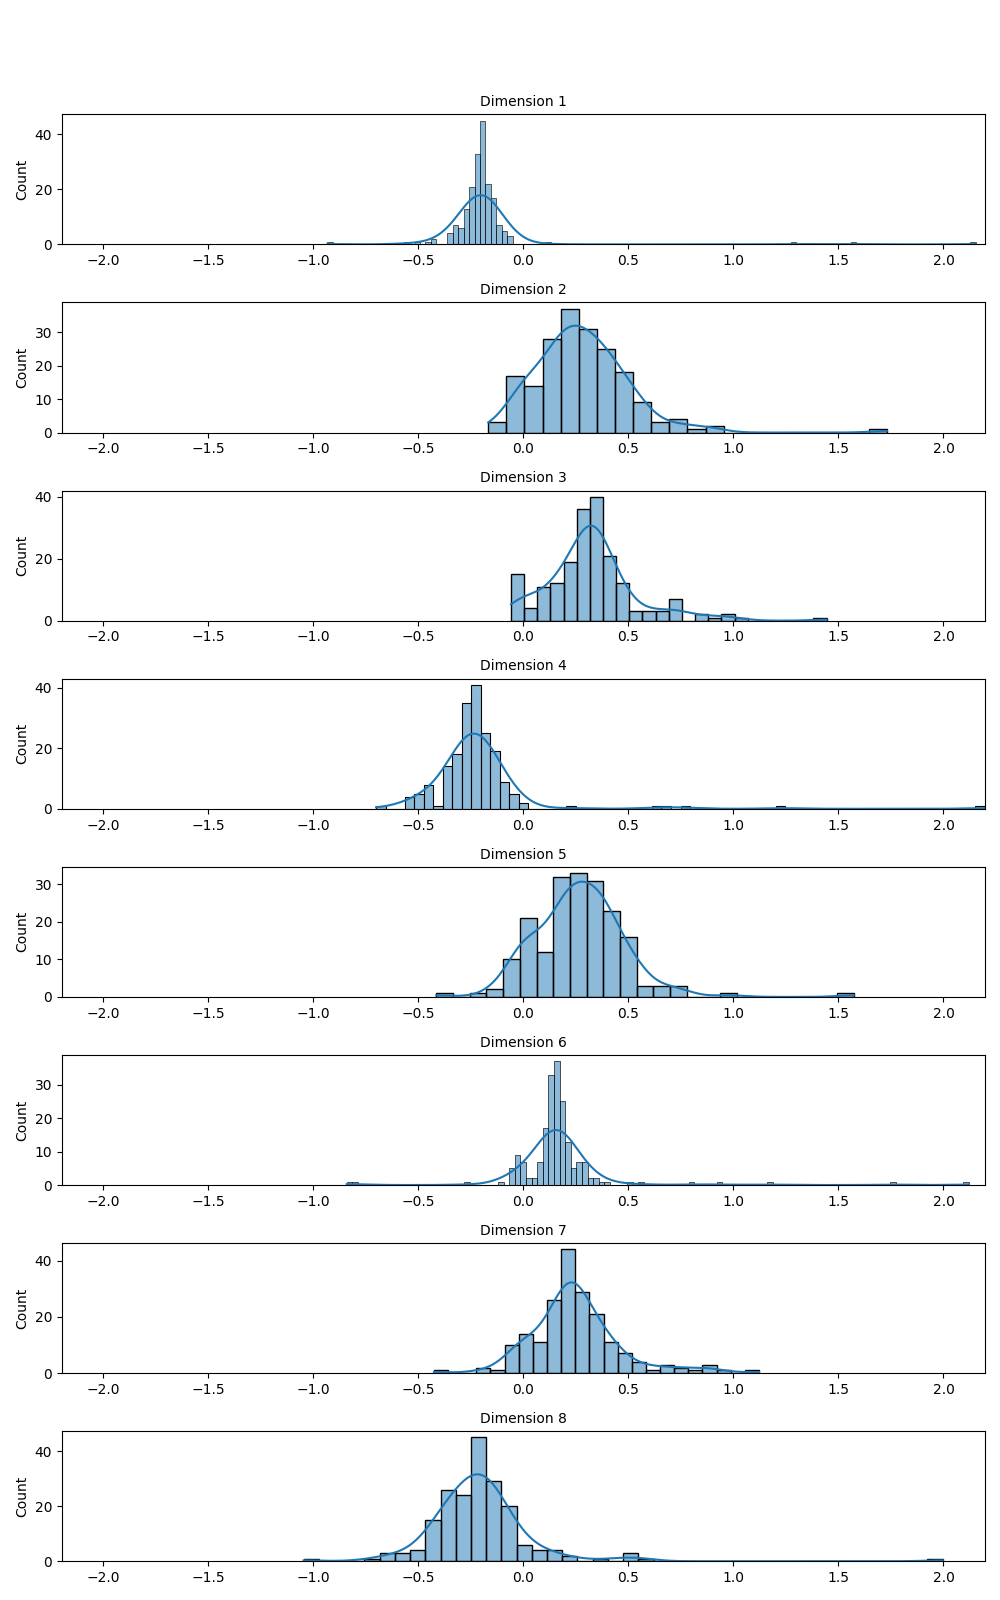
\includegraphics[width=0.5\textwidth]{final_latent_plot.png}  % Change 'image.png' to the name of your image file
    \caption{Box plots of latent dimensions.}
    \label{fig:latentspaces}
\end{figure}
\clearpage 
\vspace{1em}
\noindent
We note that although the shape of each latent dimension is approximately standard normal, the exact mean and variance varies between dimensions. This is because we lowered the weighting of the KL divergence term as otherwise the model was over-regularised, causing latent space collapse (i.e. all of the generated samples looked the same).\\\\
Standard practice in VAE's is to simply sample from the prior distribution $z\sim \mathcal{N}(\mathbf{0}, \boldsymbol{\mathbb{I}})$ in order to generate novel samples, however, in light of the above latent dimension projections, we decided to sample from a multivariate gaussian $z \sim \mathcal{N}(\boldsymbol{\mu}, \boldsymbol{\Sigma})$ where $\boldsymbol{\mu}_i$ is simply the mean of the $i^{th}$ dimension's latent embeddings, and $\boldsymbol{\Sigma}$ is a diagonal covariance matrix where $\boldsymbol{\Sigma}_{ii}$ is the variance of the $i^{th}$ dimension's latent embeddings.\\\\
After the CVAE was trained, 100 000, 30 day paths were simulated. This was done by using the CVAE to generate 6 5-day log-signatures, each conditioned on the previous time-period's log-signature. The pseudo-code below describes the exact methodology followed:\\
\begin{algorithm}[H]
\caption{Log-signature Generation}
\begin{algorithmic}[1]
    \STATE \texttt{log\_signature\_paths} $\gets$ \texttt{[]}
    \FOR{$i = 1$ \TO $100{,}000$}
        \STATE \texttt{conditional} $\gets$ \text{log-signature of the last path in training data}
        \STATE \texttt{path} $\gets$ \texttt{[]}
        \FOR{$j = 1$ \TO $6$}
            \STATE Sample $\mathbf{z} \sim \mathcal{N}(\boldsymbol{\mu}, \boldsymbol{\Sigma})$
            \STATE \texttt{x} $\gets$ \text{CVAE\_Decoder}($\mathbf{z}$, \texttt{conditional})
            \STATE \texttt{conditional} $\gets$ \texttt{x}
            \STATE Append \texttt{x} to \texttt{path}
        \ENDFOR
        \STATE Append \texttt{path} to \texttt{log\_signature\_paths}
    \ENDFOR
\end{algorithmic}
\end{algorithm}

\subsubsection{Inversion}
The iisignature package \cite{iisignature} was then used to exponentiate each log-signature into a signature, and then the Signatory package \cite{kidger2021signatory}  was used to convert these signatures into time-series paths. It must be noted that the inversion of path signatures back into real-world paths is highly nontrivial, and the Signatory package is limited to returning paths of length = depth + 1, where depth is the depth of the signature produced. This was in fact why we generated paths of length 5, as taking signatures of higher depths was computationally too expensive. \\\\
The full algorithm for the path inversion is as follows:\\
\begin{algorithm}[H]
\caption{Signature Inversion}
\begin{algorithmic}
    \STATE \texttt{paths} $\gets$ \texttt{[]}
    \FOR{$i = 1$ \TO $100{,}000$}
        \STATE \texttt{path} $\gets$ \texttt{[]}
        \FOR{$j = 1$ \TO $6$}
           \STATE \texttt{signature} $\gets$ \text{logsig\_to\_sig}(\texttt{log\_signature\_paths[i][j]})
           \STATE \texttt{6\_day\_path} $\gets$ \text{signature\_inversion(\texttt{signature})}
           \IF{$i>1$}
               \STATE Shift \texttt{6\_day\_path} to have its first value equal the previous  \texttt{6\_day\_path}'s final value
           \ENDIF
           \STATE \texttt{5\_day\_path} $\gets$ \texttt{6\_day\_path[1:]}
           \STATE Append \texttt{5\_day\_path} to \texttt{path}
        \ENDFOR
    \ENDFOR
\end{algorithmic} 
\end{algorithm}

\subsection{Deep Hedging}
\subsubsection{Data}
The data used to train the Deep Hedger is of course the paths generated using the CVAE. 100 000 paths were simulated and this data was randomly split into training, validation and testing datasets using a 70/20/10 split.

\subsubsection{Feed-Forward Neural Network Architecture}
The simple feed-forward neural network takes in as input the two stock's current prices and the time to maturation of the option, ie: 
\begin{align*}
    \text{input} = \left[S^{1}_{t}, S^{2}_{t}, T-t\right]
\end{align*}
and outputs $\phi$, the holdings of the two stocks in the portfolio at time $t$, ie: 
\begin{align*}
    \text{output} = \boldsymbol{\phi}_{t} = \left[\phi^{1}_{t}, \phi^{2}_{t}\right].
\end{align*}

\subsubsection{LSTM Architecture}
As described, the LSTM takes in as input a sequence of inputs. In our case this is the sequence of stock prices associated with our period of training alongside the time to maturation of the option, ie:
\begin{align*}
    &\text{input} = \mathbf{x}\\
    &\mathbf{x} = [\mathbf{x}_0,...,\mathbf{x}_{T-1}]\\
    &\mathbf{x}_t = \left[S^{1}_{t}, S^{2}_{t}, T-t\right]
\end{align*}
Note that the last day of stock data (i.e. the day of maturation) does not get included as an input, as we can only make trades on days leading up to but not including the day of maturation of the option.

\subsubsection{Loss function}
Prior to training, the option prices $H_{i} = [H_{0}, H_{i,1}, H_{i,2},...,H_{i,T}]$ were calculated for each input path $1 \leq i \leq$ 100 000 as informed by the Black-Scholes equation as described in \ref{final Ht formula}, where $H_{i,T} = 100 \times \text{max}\left\{\frac{S^{1}_{T}}{S^{1}_{0}}, \frac{S^{2}_{T}}{S^{2}_{0}}\right\}$ is the actual payoff of the $i^{th}$ path. Note that the option price $H_0$ is the same for all paths, as this is the price the actual option is sold at at time $t=0$ and is thus path independent.
\\\\
For each input path, the loss was calculated to be the sum of squared error between the changes in the value of our portfolio and the changes in the option's price, namely:
\begin{align}
    loss_i &= \sum_{t=1}^{T}\left[\Delta V_{i,t} - \Delta H_{i,t}\right]^2\\
    &=\sum_{t=1}^{T}\left[\left(V_{i,t}-V_{i,t-1}\right)-\left(H_{i,t}-H_{i,t-1}\right)\right]^2\\
\end{align}
where 
\begin{align}
    V_{i,t} &= V_{i,0} + \sum_{j=1}^{t} (\Delta \boldsymbol{ S}\cdot \boldsymbol{\phi}_{j})\\
    &= H_{0} +\sum_{j=1}^{t} \left[\left(S_{j}^1-S_{j-1}^1\right) \phi_{j,1} + \left(S_{j}^2-S_{j-1}^2\right)\phi_{j,2}\right] 
\end{align} is the value of our portfolio at time $t$ as governed by the trading strategy given by our neural network.
\\\\
This choice of loss function is naturally motivated by the fact that if the changes in our portfolio's value closely tracks that of the changes in the true option's value, then the final value's should be similar.


\subsubsection{Hyperparameter Search}
For both the Feed-Forward and LSTM models, a hyperparameter search was conducted using the Optuna library \cite{optuna_2019}, using the validation loss on the 20 000 validation set as a means of determining optimal hyperparmeters. \\\\
Optuna uses a median criterion for pruning unpromising runs. More specifically, if the validation loss of a run after epoch $k$ is more than the median loss of all previous runs after epoch $k$ then that run will be stopped prematurely so that more promising runs can be explored. A possible issue that arises from this is that different runs have different learning rates, and so a certain run might be doing worse near the beginning of training but then eventually end up outperforming another run later on. We also have the issue that if somehow the first few runs performed relatively well, then many future runs will be culled off which might limit proper exploration of the hyperparameter space. In order to try combat these shortcomings, we only allowed pruning to take place after 10 full runs had occurred, and thereafter only after 10 epochs of training (per run).\\\\

\subsubsection{Feed-Forward Hyperparameters}
We decided to do 500 runs each of 100 epochs in order to effectively explore the relatively large search space in a reasonable amount of time given our computational and time constraints. The hyperparameters, their ranges, as well as the optimal values found are presented in the table below. Note that continous ranges are depicted with [ ], whilst finite, categorical ranges are depicted with $\{\}$.
\label{Feedforward hyperparameters}
\begin{table}[h]
\centering
\begin{tabular}{|c|c|c|}
\hline
\textbf{Hyperparameter} & \textbf{Range/Values Considered} &\textbf{Optimal Value Found} \\
\hline
activation & \{ReLU, Tanh, LeakyReLU\}&LeakyReLU\\
learning rate & [1e-5, 1e-2]& 5.377e-3\\
batch size & \{64, 256, 1024, 4096, 8192\}&8192\\
optimizer & \{Adam, SGD\} & Adam\\
l1 regularisation &[0, 1e-2]&3.643e-7\\
l2 regularisation &[0, 1e-2]& 7.399e-3\\
number of layers & [1,5] & 1\\
width layer 1 & [32, 512] &169\\
dropout layer 1 &[0, 0.3]&2.371e-1\\
\hline
\end{tabular}
\caption{Hyperparameter search space and optimal hyperparameters found for Feed-Forward Hedger}
\label{tab:hyperparams}
\end{table}\\
We note that all optimal values found fall reasonably within the ranges considered, except that of the batch size, whose optimal value was the upper bound of the range considered. When the batch size was increased beyond 8192 we had errors with GPU memory allocation, so this is the size we settled on.

\subsubsection{LSTM Hyperparameters}
Before conducting a full hyperparameter search for the LSTM we trained a non-tuned LSTM as a sanity check to see if there was any potential benefit in using a LSTM architecture over a standard feed-forward one. This model will henceforth be referred to as the Untuned LSTM model. The (randomly chosen) hyperparameters for this model are captured in the table below:
\begin{table}[h]
\centering
\begin{tabular}{|c|c|}
\hline
\textbf{Hyperparameter} & \textbf{Value}  \\
\hline
learning rate & 0.001\\
batch size & 2048\\
optimizer & Adam\\
l1 regularisation &0\\
l2 regularisation &0\\
number of layers & 2\\
width layer 1 & 128\\
width layer 2 & 128\\
dropouts &0\\
\hline
\end{tabular}
\caption{Hyperparameters for Basic LSTM}
\label{tab:hyperparams}
\end{table}\\
Due to the increased complexity and consequently training time of the LSTM vs standard feed-forward models, we had to reduce the number of runs and epochs over which the hyperparameter tuning was done. Thus the LSTM hyperparameter tuning took place for 100 runs each over 50 epochs.

\label{LSTM hyperparameters}
\begin{table}[h]
\centering
\begin{tabular}{|c|c|c|}
\hline
\textbf{Hyperparameter} & \textbf{Range/Values Considered} &\textbf{Optimal Value Found} \\
\hline
learning rate & [1e-5, 1e-2]& 1.334e-4\\
batch size & \{64, 256, 1024\}&1024\\
optimizer & \{Adam, SGD\} & Adam\\
l1 regularisation &[0, 1e-2]&3.690e-5\\
l2 regularisation &[0, 1e-2]& 3.380e-3\\
number of layers & [1,5] & 1\\
width layer 1 & [32, 512] &432\\
dropout layer 1 &[0, 0.3]&9.033e-1\\
\hline
\end{tabular}
\caption{Hyperparameter search space and optimal hyperparameters found for LSTM Hedger}
\label{tab:hyperparams}
\end{table}\\

\subsubsection{Final Training}
The Feed-Forward, Tuned LSTM and Untuned LSTM models were all then trained for 1000 epochs on the full 90 000 non-test pseudo-generated paths using the hyperparameters as found above.

\subsubsection{Testing Hedging Performance}
Our hypothesis is that the Deep Hedging Models will outperform Black-Scholes in the hedging of financial instruments. In order to test this hypothesis we need to use both Black-Scholes and our trained models to make trades in order to hedge against the option of interest. To this end we have two sets of test results. Firstly we use all the models to trade on the 10 000 pseudo-generated test paths and compare the profit and losses (PNLs) across all these paths. The PNL for a single path is calculate as:
\begin{align}
    \text{PNL} = V_T-H_T
\end{align}
i.e. it is the difference of the final value of our portfolio under our trading strategy vs the final value of the option.\\\\
For the Black-Scholes model, the hedging strategy used is simply that as informed by \ref{final Ht formula}. i.e. At every time $t$, we simply have our holdings for stock 1 and stock 2 being
\begin{align}
    \text{holdings}_{t} = \left[\Phi\left(d_1^{\frac{i}{j}}(t)\right), \Phi\left(-d_2^{\frac{i}{j}}(t)\right)\right].
\end{align}\\\\
For all the neural networks, our holdings at time $t$ are simply the output of the neural network given the input up to time $t$, 
\begin{align}
    \text{holdings}_{t} = \text{model}(\text{input}_{t}).
\end{align}
The very final test of the models is how each performs on the true real-world 30 day stock path. Since this would only result in a single PNL, to get a better idea of how well each model tracked the price of the option we additionally calculated the Mean-Squared-Error between the changes in each model's portfolio value, and the changes in the actual option's price:
\begin{align}
    \text{MSE} = \frac{1}{30}\sum_{t=1}^T \left[\Delta V_t - \Delta H_t\right]^2
\end{align}
\newpage
\section{Results}
\subsection{Path Generation}
\subsubsection{Training Loss}
The plots below shows the Mean Squared Error (MSE) loss, Total loss and KL koss of the VAE over the 20 000 epochs of training. Please note that the MSE and Total losses were plotted on a log-scale, whilst the KL loss was plotted on a linear scale.

\begin{figure}[H]  % 'H' for placing the figure exactly here
    \centering
    \begin{minipage}[t]{0.49\textwidth}
        \centering
        \includegraphics[width=\textwidth]{VAE_MSE_loss_plot.png}
        \caption{VAE MSE loss}
        \label{fig:mse_loss}
    \end{minipage}
    \hfill
    \begin{minipage}[t]{0.49\textwidth}
        \centering
        \includegraphics[width=\textwidth]{VAE_total_loss_plot.png}
        \caption{VAE Total loss}
        \label{fig:total_loss}
    \end{minipage}
\end{figure}

\begin{figure}[H]  % 'H' for placing the figure exactly here
    \centering
    \includegraphics[width=0.6\textwidth]{VAE_KL_loss_plot.png}
    \caption{VAE KL loss}
    \label{fig:kl_loss}
\end{figure}
\noindent We note that the MSE loss (and consequently the total loss) quickly saturates, and the only thing really changing during later epochs is the slow decrease in KL divergence loss as the neural network attempts to coerce the latent space's distribution to more closely resemble that of a standard Gaussian.\\\\

\subsubsection{Distribution Similarity}
The effectiveness of our hedger depends upon the ability of our VAE to generate samples from the same distribution as the true sample path.\\\\
As a sanity check, we went through the historical stock data used to train the VAE, and then used the VAE to generate each 5-day window, conditioned on the previous real 5-day window in the training data. The real historical paths and our new generated paths were then plotted against each other:
\begin{figure}[H]  % 'H' places the figure exactly here
    \centering
    \includegraphics[width=1\textwidth]{Original_vs_Generated.png}  
    \caption{Original and Generated Stock paths over 1000 day historical period}
    \label{fig:apple_image}
\end{figure}
\noindent
We see that both generated paths end up reasonably close to the final prices of the true paths. More importantly, our generation effectively captures qualities of the joint distribution of the stocks, such as correlation and covariance, which can be seen by the fact that similar movements happen in each stock over similar periods of time. This similarity in movement is exactly what is seen in the original stocks, and is what would be expected of two stocks representing companies from the same industry (in this case the tech industry). 

\subsubsection{Distribution of Gains}
In the context of Hedging, we are mainly concerned with ensuring that the distribution captured by the VAE is representative of the true gains and losses of the real-world data. This is especially true in our particular option's case, where the value of the option is a direct consequence of the movements of the two stocks relative to their initial price. Again we used the 200 5-day generated samples as above, but this time compared the generated movements (i.e. final value - initial value) of our generated samples with those of the real-world 5-day movements. This comparison is captured in the plots below:

\begin{figure}[H]  % 'H' for placing the figure exactly here
    \centering
    \begin{minipage}[t]{0.49\textwidth}
        \centering
        \includegraphics[width=\textwidth]{apple_gains_2.png}
        \caption{Apple Gains}
        \label{fig:Original vs Generated Gains for Apple Stock}
    \end{minipage}
    \hfill
    \begin{minipage}[t]{0.49\textwidth}
        \centering
        \includegraphics[width=\textwidth]{microsoft_gains_2.png}
        \caption{Microsoft Gains}
        \label{fig:Original vs Generated Gains for Microsoft Stock}
    \end{minipage}
\end{figure}
\noindent
We see that the gains for each stock are similar, although the original movements for both stocks is more spread out, which might have negative implications for the robustness of our hedger.
\subsubsection{Kolmogorov-Smirnov Test}
The two-sample Kolmogorov-Smirnov (K-S) test tests if two empirical distributions are different to one another. The theory motivating the effectiveness of the test can be found in \cite{mit_ks_test}, and a practical implementation of the test can be found in \cite{bolen2024kolmogorov}. The K-S test is a non-parametric test which compares the CDF's of the two distributions in question by finding the maximal difference in their CDF's over their support. More formally, the K-S test statistic is
\begin{align}
    D_{n,m} = \underset{x}{\sup} \left|F_{1,n}(x)-F_{2,m}(x)\right|
\end{align}
where $F_{1,n}(x)$ and $F_{2,m}(x)$ are the empirical CDF's of the two distributions, and $n$ and $m$ the number of samples from each. For large samples, the null hypothesis is rejected at level $p=0.05$ when
\begin{align}
    D_{n,m} \geq 1.358 \sqrt{\frac{n+m}{n m}}.
\end{align}
The null hypothesis for the test is that the distributions are the same, i.e., when comparing two random variables $X$ and $Y$, we have that
\begin{align*}
    &H_0: F_X = F_Y\\
    &H_1: F_X \neq F_Y.
\end{align*}
We performed K-S tests between the generated and original gains for both of the stocks. The results the two tests are captured in the table below:
\begin{table}[h!]
    \centering
    \begin{tabular}{|c|c|c|}
        \hline
        & \textbf{KS Test-Statistic} & \textbf{p-value} \\ 
        \hline
        \textbf{Apple Stock} & 0.1031 & 0.2545 \\ 
        \hline
        \textbf{Microsoft Stock} & 0.0515 & 0.9596 \\
        \hline
    \end{tabular}
    \caption{p-values from two K-S tests for Apple and Microsoft stocks}
\end{table}\\
\noindent
We see that neither p-values are near the threshold of 0.05, and thus we cannot say that the samples come from different distributions. 
\\\\
Although this test does not ``prove" that the two distributions are the same, it at least tells us that there is not enough evidence to suggest that the distributions are different.
\subsubsection{Conditional Generation}
A major proponent of the generation is that we are attempting to sample from a conditional distribution rather than an unconditional one. In order to test whether or not this conditioning was effective, we used the true and generated 5 day windows over the period of the training data. We shifted all 5 day windows to begin and zero, and then calculated the MSE between the generated 5 day window to that of the true 5 day window. We then randomly chose another real-world 5 day window from the training data, also shifted down to zero, and calculated the MSE between this randomly chosen path and the true path. Finally we took the mean of the real vs generated MSEs and the mean of the real vs random MSEs. The table below compares the MSEs for both path 1 and path 2, and then the final overall MSEs across both paths:
\begin{table}[h!]
    \centering
    \begin{tabular}{|c|c|c|}
        \hline
        & \textbf{Real vs Generated} & \textbf{Real vs Random} \\ 
        \hline
        \textbf{Path 1 MSE} & 17.7778 & 24.2246 \\ 
        \hline
        \textbf{Path 2 MSE} & 56.3932 & 76.4926 \\
        \hline
        \textbf{Total MSE} & 37.0855 & 50.3586\\
        \hline
    \end{tabular}
    \caption{MSEs of Real vs Generated and Real vs Random subpaths}
\end{table}\\
\noindent
We see that on average the conditionally generated paths are significantly closer to the real paths than the real paths to a randomly selected path. This indicates that our VAE has effectively learnt the conditional distribution.

\subsubsection{Generating Future Samples}
Our main interest is simulating both stocks 30 days into the future, as this is the period over which we will be trading in an attempt to replicate the option value.
\\\\
The plots on the next page show 1000 generated samples for both the Apple and Microsoft stock prices over this 30 day period.

\begin{figure}[H]  % 'H' places the figure exactly here
    \centering
    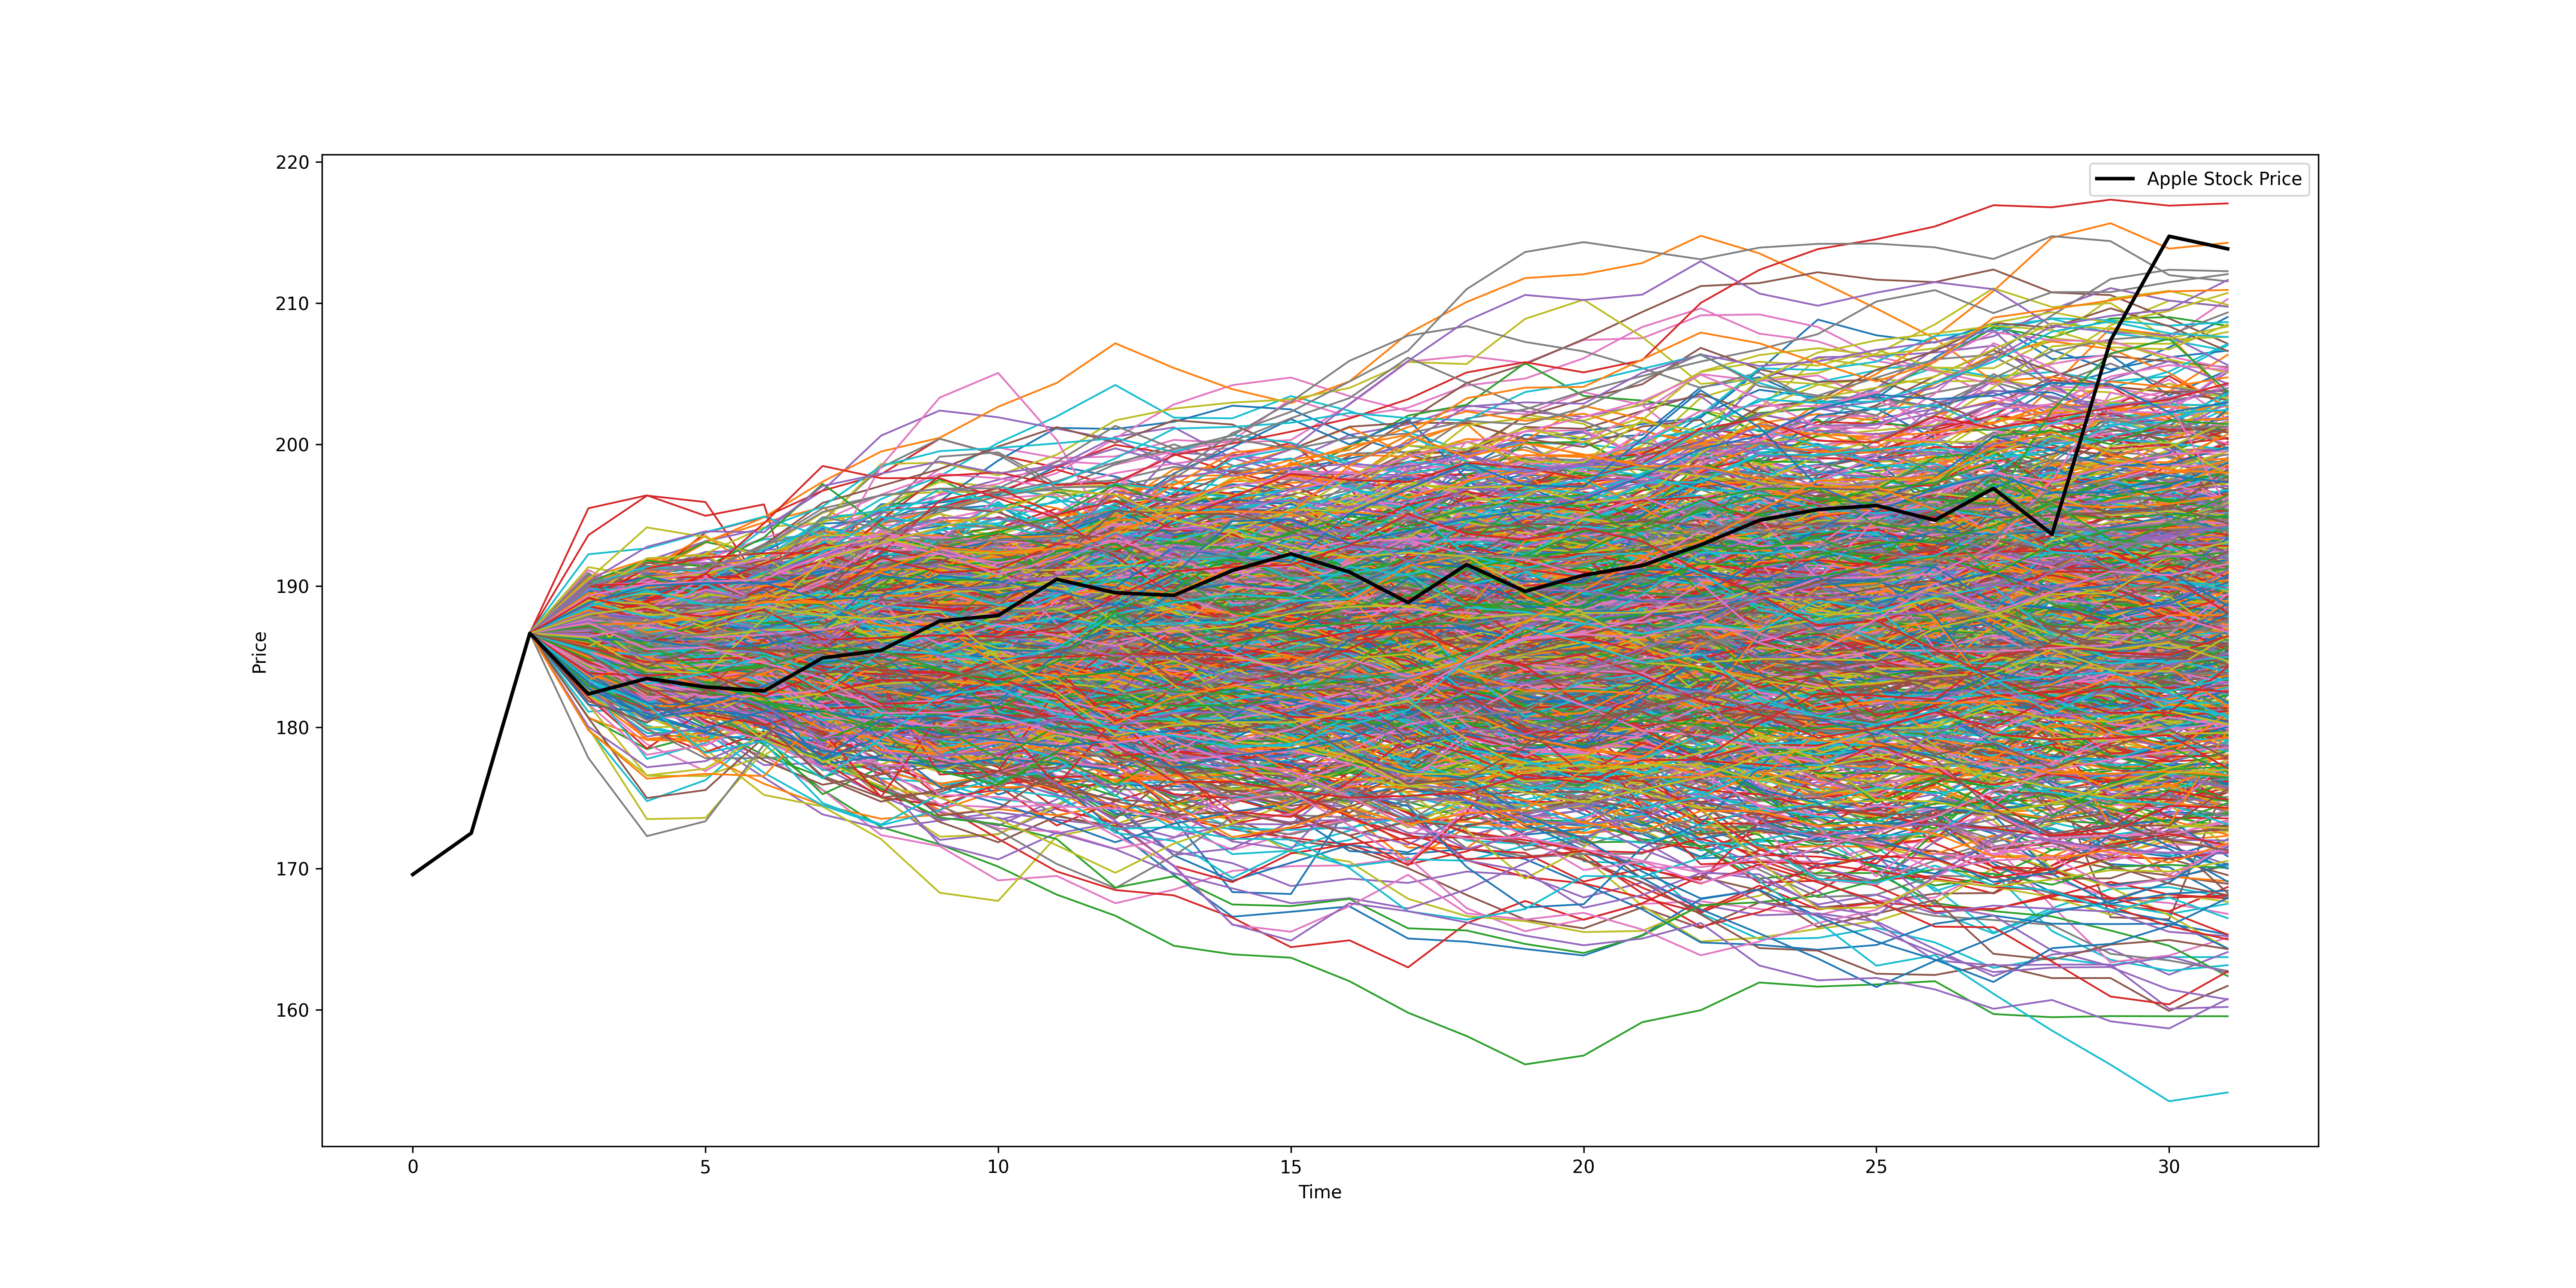
\includegraphics[width=0.8\textwidth]{tail_end_original_and_generated_path_Apple_Stock.png}  
    \caption{Original and Generated Apple Stock paths}
    \label{fig:apple_image}
\end{figure}

\vspace{0.5cm}  % Adds some space between the figures

\begin{figure}[H]  % 'H' places the figure exactly here
    \centering
    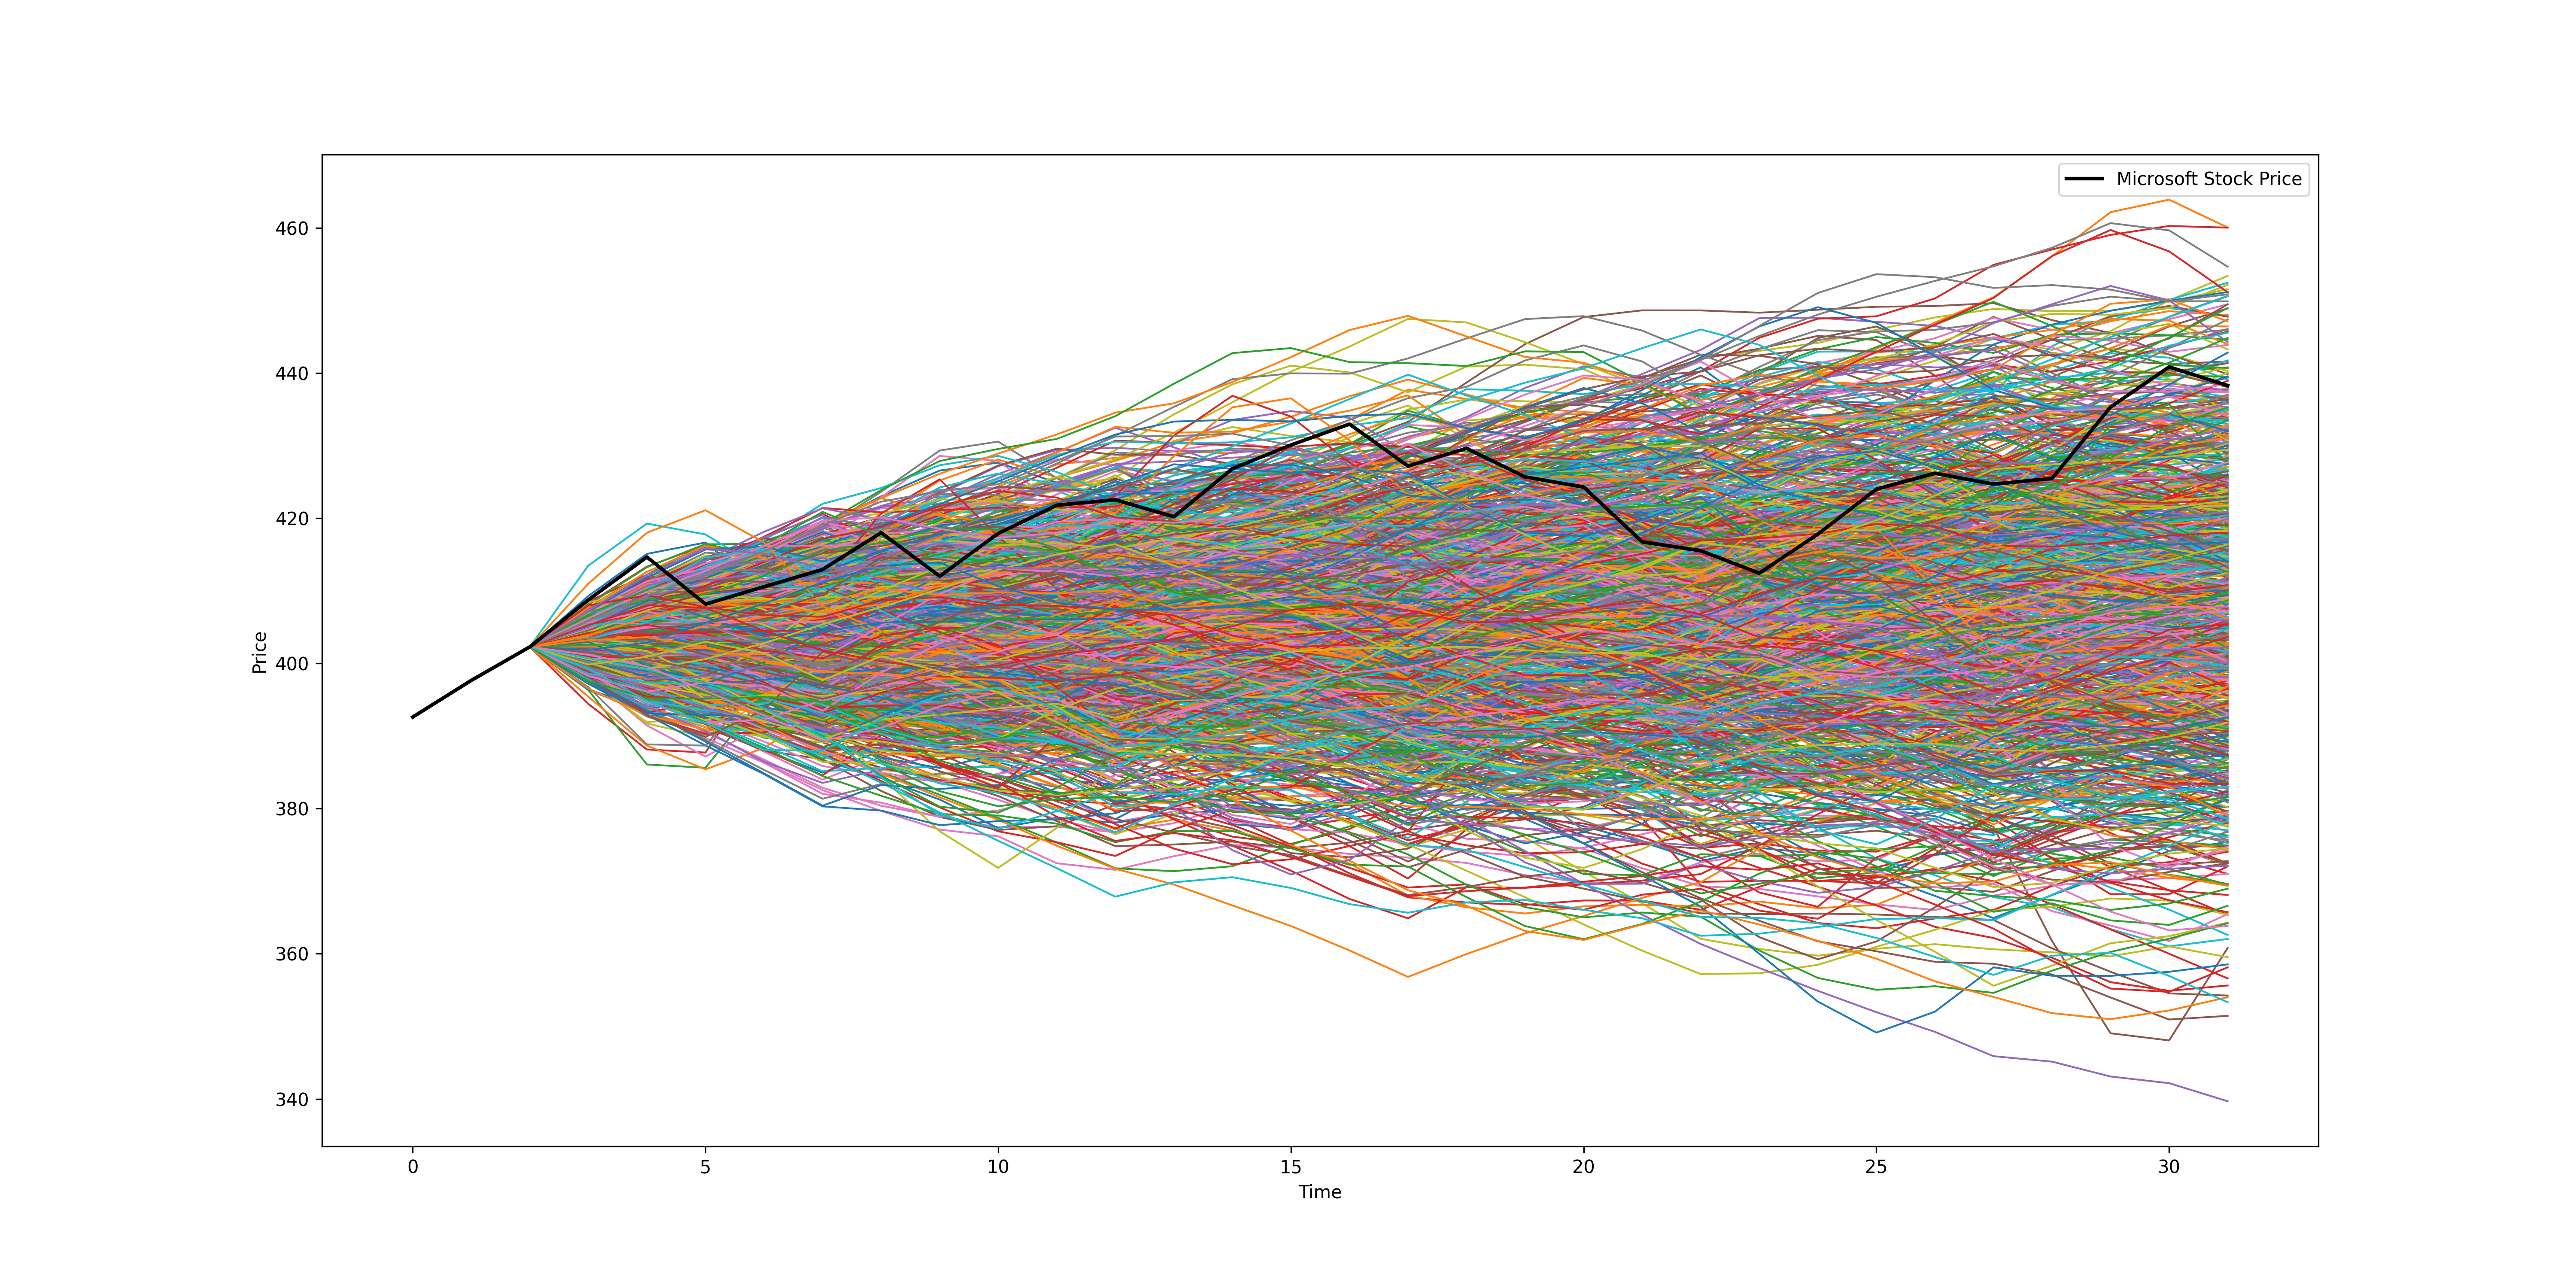
\includegraphics[width=0.8\textwidth]{tail_end_original_and_generated_paths_Microsoft_Stock.png}  
    \caption{Original and Generated Microsoft Stock paths}
    \label{fig:microsoft_image}
\end{figure}
\noindent
We note that the generated paths for both stocks have a good spread whose range appears to be realistic when compared to the real-world data in the 30 day generated period.
\newpage

\subsection{Deep Hedging}

\subsubsection{Feed-Forward Loss curves}
For the Feed-Forward network, we recorded both the training and test set loss at each epoch of training, depicted in the log-scaled plot below:
\begin{figure}[H]  % 'H' places the figure exactly here
    \centering
    \includegraphics[width=0.8\textwidth]{ffNN_loss_plot.png}  
    \caption{Feed-Forward Training and Test Loss Curves}
    \label{fig:ffNN_loss_curves}
\end{figure}
\noindent
We see that there are clear spikes in loss which gradually decrease over time. There are many possible explanations to this, one of which is the way in which updates to the model's parameters occur in batches. More specifically, within an epoch we update the model $k$ times, where $k$ is the number of batches in our training set. The loss used to make an update to the parameters of the model is the mean loss of a single batch. Now, due to the random allocation of training samples to batches, if many of the samples in a single batch happen to be outliers in the data or samples which the model struggles to fit, the loss incurred by this batch will be very large when compared to the other batches and consequently the effect on the change in the model parameters will be large (since the size of update is proportional to the loss incurred). This means the model will likely over-correct to try and accommodate these samples, meaning that in the next batch or epoch the loss could spike as the model is much worse at predicting the output on average. Due to the use of a momentum optimiser such as Adam, the over-correcting nature of these updates decreases over time, accounting for the fact that the peaks of these spikes decreases.\\\\
We also note that the test losses decrease almost identically to the training, which helps give us confidence that the hyperparameters found do indeed help the model generalise to unseen data.

\subsubsection{Tuned LSTM Loss Curves}
Similarly, we plotted the training and test losses for the Tuned LSTM, but this time on a linear scale due the comparatively small range.
\begin{figure}[H]  % 'H' places the figure exactly here
    \centering
    \includegraphics[width=0.8\textwidth]{LSTM_loss_plot.png}  
    \caption{Tuned LSTM Training and Test Loss Curves}
    \label{fig:LSTM_loss_curves}
\end{figure}
\noindent
We see that both the training and test losses quickly saturate and then fluctuate around a point just above 0.10. This indicates much further training would not have increased the performance of the model, and that once more the hyperparameters chosen ensure that the model is not overfitting to the training data.

\subsubsection{Untuned LSTM Loss Curves}
Again we plotted the training and test loss curves for the Untuned LSTM model on a linear scale:
\begin{figure}[H]  % 'H' places the figure exactly here
    \centering
    \includegraphics[width=0.8\textwidth]{untuned_LSTM_loss_plot.png}  
    \caption{Untuned LSTM Training and Test Loss Curves}
    \label{fig:LSTM_loss_curves}
\end{figure}
\noindent
This is the most promising of all three loss curves, with the minimum training and test losses achieved being lower than that of the Feed-Forward and Tuned LSTM models.  training and test losses decrease in similar fashions. The training loss curve decreases in a much more consistent and linear fashion than the other loss curves, and looks like it would continue to decrease if we continued training, however we note that the test loss begins to increase near the end of the 1000 epochs. This indicates that the model is capable of overfitting to the training data, which makes sense given that the Untuned LSTM had no regularisation applied to it. That being said, the fact that we stopped ``early'' (before the training loss asymptoted) is in itself a form of regularisation, and the fact that the test loss only just began to increase near the end of the 1000 epochs indicates that this model would still perform well on unseen data.

\subsubsection{Hedging Performance (Generated Paths)}
We found the PNLs for all models under the 10 000 generated test paths.\\
The mean and variance of these (PNLs) are compared to those made by a delta-hedging trading strategy informed by Black-Scholes in the table below:
\begin{table}[h!]
    \centering
    \begin{tabular}{|c|c|c|c|c|}
        \hline
        & \textbf{Black-Scholes} & \textbf{Feed-Forward NN} & \textbf{LSTM NN} & \textbf{Untuned LSTM} \\ 
        \hline
        \textbf{Mean(PNLs)} & 1.3481 & 0.1780 & 1.2922 & 0.0575\\ 
        \hline
        \textbf{Variance(PNLs)} & 0.4476 & 4.9558 & 4.8277 &1.7408\\
        \hline
    \end{tabular}
    \caption{Comparison of different model's mean and variance of PNLs on Generated Paths}
\end{table}\\
\noindent
We see that all the neural networks beat Black-Scholes on average, with the feed-forward neural netwok getting a mean PNL an order of magnitude closer to 0, and the Untuned LSTM being two orders of magnitude closer, however for all models Black-Scholes clearly beats them in its variance.\\\\
Counter-intuitively, the tuned LSTM has the worse mean of all the trained models, however as mentioned, due to time and computation constraints we were unable to run many trials over many epochs when attempting to find the optimal hyperparameters. Thus, we likely just never found the optimal region during our search. The improved performance of the Untuned LSTM indicates that more complex models might very well lead to better performance, as the Untuned LSTM had no form of regularisation and had two layers as opposed to the single layer found to be optimal during the hyperparameter search. This is however at least promising, as it indicates that even better results are likely achievable with this architecture.  
\\\\
To help visualise the difference in mean and spread of the PNLs, we plotted the PNLs of the Black-Scholes model versus those of the Untuned LSTM model:
\begin{figure}[H]  % 'H' places the figure exactly here
    \centering
    
\includegraphics[width=0.8\textwidth]{BS_LSTM_PNLs.png}  
    \caption{BS vs Untuned LSTM PNLs}
    \label{fig:BS_LSTMS_PNLs}
\end{figure}
\noindent

\subsubsection{Hedging Performance (Final Test)}
The final test statistics (as described in the methodology section) for all the models on the real-world 30 day test set are shown in the table below: 
\begin{table}[h!]
    \centering
    \begin{tabular}{|c|c|c|c|c|}
        \hline
        & \textbf{Black-Scholes} & \textbf{Feed-Forward NN} & \textbf{LSTM NN} & \textbf{Untuned LSTM} \\ 
        \hline
        \textbf{MSE($\Delta V_t-\Delta H_t$)}&1.8570 & 0.7452&0.7262 &1.3326\\
        \hline
        \textbf{Final PNL} &-1.3963 &-4.8725 &-4.4570 & 0.5634\\
        \hline
    \end{tabular}
    \caption{Comparison of model performance for final real-world test set}
\end{table}\\
\noindent
We see that the feed-forward and Tuned LSTM model portfolios best track the option price on average, however end up having worse PNLs at the time of maturity. This means that the Black-Scholes and Untuned LSTM models made errors earlier on in trading, but then made up for them near the end of training, resulting in better final PNLs. The Untuned LSTM had the best overall PNL, again displaying that it could be used to competitively hedge this option.\\\\
It must be noted that the real-world 30 day test path is actually just one sample from the conditional distribution of possible future paths given the past, so these statistics are not truly representative of how these models would perform on average, hence why we additionally did testing on the pseudo-generated paths.

\newpage
\section{Discussion}
\subsection{Generation}
Our findings agree with the overwhelming literature that VAEs can be effectively used as a generative architecture. Our findings also agree with that of the literature \cite{buehler2020data}, \cite{buehler2020generating}, \cite{stangroom2023deephedging} in that we can effectively use signatures and VAEs to simulate financial markets in low data environments. Our work also expands upon previous literature in that we simulated the movements of two stocks to effectively generate paths coming from a joint-distribution so that we could hedge a basket option as opposed to a more generic single-stock barrier option.
\subsection{Hedging}
With regards to the use of Deep Neural Networks (DNNs) to govern hedging strategies, our findings only partially agree with that of the existing literature \cite{stangroom2023deephedging} and Buehler et al. \cite{buehler2019deep} in that the trading strategies governed by DNNs can indeed outperform more traditionally informed strategies when hedging a European style option. The findings are only partially agreeable as we found issues of variability in our study which were not found in these other studies.
\newpage

\section{Conclusion}
We set out to see whether a DNN could trade assets underlying an Exotic European Basket option so as to replicate the value of the contingent claim, and whether it could do this better than the traditional methods of Black-Scholes.\\\\
In order to do this we first attempted to learn the underlying stocks' joint conditional distributions with a VAE. The results of our generation process showed promise in that this approach can effectively learn such distributions, even in relatively low-data environments.
\\\\
On the actual use of DNN for hedging we had mixed results with our models attaining better mean PNLs on generated paths, but having higher variance than those of the Black-Scholes model. The findings are however promising in that they indicate that with better compute and time, the models could be improved to eventually beat Black-Scholes on both metrics. As such, we conclude that there is clear potential for DNNs to be used to solve the short-comings of the Black-Scholes equations, in that they may more accurately be able to replicate basket price options in incomplete, discrete-time markets. 
\newpage

\section{Improvements and Further Research}
Given that this was an Honours Project, the scope of this paper is greatly limited. Countless obstacles were met throughout the project and countless mistakes made. The author did their best to remedy these, but it would be against the scientific endeavour not to mention some of the short-comings of this paper. Additionally, the author came across many open questions that they believe would be interesting to explore in greater detail further down the line. This sections aims to address and expand upon both the short-comings and future avenues of exploration.

\subsection{Path Signature Inversion}
As has been mentioned, the inversion from a path signature back to it's original time-series data is a difficult one. In the other papers which this project mimics (\cite{buehler2020generating}, \cite{stangroom2023deephedging}), evolutionary algorithms were used in order to find the path inversions. In our case we simply used the Signatory library (\cite{kidger2021signatory}). This greatly limited us in a number of regards.\\\\
Firstly, we were not able to apply lead-lag transformations to the training data. These transformations help capture the important notion of quadratic variation and co-variation of paths (\cite{gyurko2014extracting}) and are consequently highly beneficial when attempting to learn and generate financial data. The issue is that the transformation nearly quadruples the dimensionality of the data, meaning that the size of signatures taken blows up exponentially due to the nature of the signature. As a consequence of this, the computational cost associated with inverting a signature of a lead-lagged path is massive, and it meant that we were unable to use this transformation in our implementation. \\\\
Secondly, the computational cost of signature inversion limited us to have to learn 5 day paths instead of some greater time window. In theory, larger time windows might better characterise the distribution and variance of the data, leading to better generative capabilities.
\subsubsection{Possible Solution}
The author attempted to alter the VAE to take in as input the original path and signature, and simply output the original path instead of outputting the signature. This would completely negate the need to do a signature inversion and hence overcome the issues mentioned. This approach did not work out the gate, with the VAE suffering from latent space collapse and all generated samples appearing identical. Due to time constraints we could not properly investigate if this issue is fixable, but this could offer a potential solution if further investigated.\\\\
Another possible solution is to train a wholly separate neural network to tackle the task of signature inversion, and add this to the data pipe-line.

\subsection{VAE Hyperparameter Tuning}
No validation set was used during the training of the VAE, as we did not implement a proper hyperparameter search. For the first two months of work on this project, our VAE failed miserably to generate realistic samples. This was again due to a consistent collapsing of the latent space, meaning that generated samples were nearly identical. A few of the resulting paths of failed training runs are depicted below.\\\\
\begin{figure}[ht]
    \centering
    % First row
    \begin{subfigure}{0.45\textwidth}
        \centering
        \includegraphics[width=\textwidth]{bad1.png} % Replace with your image filename
        \caption{}
        \label{fig:figure1}
    \end{subfigure}
    \hfill
    \begin{subfigure}{0.45\textwidth}
        \centering
        \includegraphics[width=\textwidth]{bad2.png} % Replace with your image filename
        \caption{}
        \label{fig:figure2}
    \end{subfigure}
    
    \vspace{1em} % Vertical space between rows

    % Second row
    \begin{subfigure}{0.45\textwidth}
        \centering
        \includegraphics[width=\textwidth]{bad3.png} % Replace with your image filename
        \caption{}
        \label{fig:figure3}
    \end{subfigure}
    \hfill
    \begin{subfigure}{0.45\textwidth}
        \centering
        \includegraphics[width=\textwidth]{bad4.png} % Replace with your image filename
        \caption{}
        \label{fig:figure4}
    \end{subfigure}
    
    \caption{Failed VAE generations}
    \label{fig:grid}
\end{figure}\\
\noindent
Once we finally managed to resolve these issues, we no longer had time to perform a proper hyperparameter search and validation analysis.
\subsubsection{Solution}
The solution to this is of course to perform a proper proper hyperparameter search and validation analysis.

\subsection{Trading}
In reality performing trades of financial instruments comes at a cost. We did not account for this in our model designs but this would be highly important in reality. This reality is also not captured in the frictionless market assumption of Black-Scholes, so in fact if we were able to effectively account for transaction costs in our models, their performance relative to Black-Scholes would likely be boosted greatly.
\subsubsection{Possible Solution}
A possible solution to this would be to include a penalty term in the loss functions of the hedging neural networks which penalises the change in holdings from one time-point to another, as this would help limit the number of transactions of the underlying assets made.

\subsection{Is Generation Necessary?}
As was pointed out by the supervisor of the project, Dr Jonathan Shock, what we are effectively doing in the project is training the neural networks on boot-strapped data, i.e. data that is estimated from the true data. Although the use of generated data gives us a nice proxy metric for the robustness of our models over future possible paths, it would be interesting to see whether or not we could simply use the true data to train a neural network to undertake the task of hedging.
\newpage

\printbibliography[title={References}, heading=bibintoc] % Prints bibliography with numbers
\end{document}

